\documentclass[]{book}
\usepackage{lmodern}
\usepackage{amssymb,amsmath}
\usepackage{ifxetex,ifluatex}
\usepackage{fixltx2e} % provides \textsubscript
\ifnum 0\ifxetex 1\fi\ifluatex 1\fi=0 % if pdftex
  \usepackage[T1]{fontenc}
  \usepackage[utf8]{inputenc}
\else % if luatex or xelatex
  \ifxetex
    \usepackage{mathspec}
  \else
    \usepackage{fontspec}
  \fi
  \defaultfontfeatures{Ligatures=TeX,Scale=MatchLowercase}
\fi
% use upquote if available, for straight quotes in verbatim environments
\IfFileExists{upquote.sty}{\usepackage{upquote}}{}
% use microtype if available
\IfFileExists{microtype.sty}{%
\usepackage{microtype}
\UseMicrotypeSet[protrusion]{basicmath} % disable protrusion for tt fonts
}{}
\usepackage[margin=1in]{geometry}
\usepackage{hyperref}
\hypersetup{unicode=true,
            pdftitle={Work of R.Vezy for the ReMIX Project},
            pdfauthor={R. Vezy},
            pdfborder={0 0 0},
            breaklinks=true}
\urlstyle{same}  % don't use monospace font for urls
\usepackage{natbib}
\bibliographystyle{apalike}
\usepackage{color}
\usepackage{fancyvrb}
\newcommand{\VerbBar}{|}
\newcommand{\VERB}{\Verb[commandchars=\\\{\}]}
\DefineVerbatimEnvironment{Highlighting}{Verbatim}{commandchars=\\\{\}}
% Add ',fontsize=\small' for more characters per line
\usepackage{framed}
\definecolor{shadecolor}{RGB}{248,248,248}
\newenvironment{Shaded}{\begin{snugshade}}{\end{snugshade}}
\newcommand{\KeywordTok}[1]{\textcolor[rgb]{0.13,0.29,0.53}{\textbf{#1}}}
\newcommand{\DataTypeTok}[1]{\textcolor[rgb]{0.13,0.29,0.53}{#1}}
\newcommand{\DecValTok}[1]{\textcolor[rgb]{0.00,0.00,0.81}{#1}}
\newcommand{\BaseNTok}[1]{\textcolor[rgb]{0.00,0.00,0.81}{#1}}
\newcommand{\FloatTok}[1]{\textcolor[rgb]{0.00,0.00,0.81}{#1}}
\newcommand{\ConstantTok}[1]{\textcolor[rgb]{0.00,0.00,0.00}{#1}}
\newcommand{\CharTok}[1]{\textcolor[rgb]{0.31,0.60,0.02}{#1}}
\newcommand{\SpecialCharTok}[1]{\textcolor[rgb]{0.00,0.00,0.00}{#1}}
\newcommand{\StringTok}[1]{\textcolor[rgb]{0.31,0.60,0.02}{#1}}
\newcommand{\VerbatimStringTok}[1]{\textcolor[rgb]{0.31,0.60,0.02}{#1}}
\newcommand{\SpecialStringTok}[1]{\textcolor[rgb]{0.31,0.60,0.02}{#1}}
\newcommand{\ImportTok}[1]{#1}
\newcommand{\CommentTok}[1]{\textcolor[rgb]{0.56,0.35,0.01}{\textit{#1}}}
\newcommand{\DocumentationTok}[1]{\textcolor[rgb]{0.56,0.35,0.01}{\textbf{\textit{#1}}}}
\newcommand{\AnnotationTok}[1]{\textcolor[rgb]{0.56,0.35,0.01}{\textbf{\textit{#1}}}}
\newcommand{\CommentVarTok}[1]{\textcolor[rgb]{0.56,0.35,0.01}{\textbf{\textit{#1}}}}
\newcommand{\OtherTok}[1]{\textcolor[rgb]{0.56,0.35,0.01}{#1}}
\newcommand{\FunctionTok}[1]{\textcolor[rgb]{0.00,0.00,0.00}{#1}}
\newcommand{\VariableTok}[1]{\textcolor[rgb]{0.00,0.00,0.00}{#1}}
\newcommand{\ControlFlowTok}[1]{\textcolor[rgb]{0.13,0.29,0.53}{\textbf{#1}}}
\newcommand{\OperatorTok}[1]{\textcolor[rgb]{0.81,0.36,0.00}{\textbf{#1}}}
\newcommand{\BuiltInTok}[1]{#1}
\newcommand{\ExtensionTok}[1]{#1}
\newcommand{\PreprocessorTok}[1]{\textcolor[rgb]{0.56,0.35,0.01}{\textit{#1}}}
\newcommand{\AttributeTok}[1]{\textcolor[rgb]{0.77,0.63,0.00}{#1}}
\newcommand{\RegionMarkerTok}[1]{#1}
\newcommand{\InformationTok}[1]{\textcolor[rgb]{0.56,0.35,0.01}{\textbf{\textit{#1}}}}
\newcommand{\WarningTok}[1]{\textcolor[rgb]{0.56,0.35,0.01}{\textbf{\textit{#1}}}}
\newcommand{\AlertTok}[1]{\textcolor[rgb]{0.94,0.16,0.16}{#1}}
\newcommand{\ErrorTok}[1]{\textcolor[rgb]{0.64,0.00,0.00}{\textbf{#1}}}
\newcommand{\NormalTok}[1]{#1}
\usepackage{longtable,booktabs}
\usepackage{graphicx,grffile}
\makeatletter
\def\maxwidth{\ifdim\Gin@nat@width>\linewidth\linewidth\else\Gin@nat@width\fi}
\def\maxheight{\ifdim\Gin@nat@height>\textheight\textheight\else\Gin@nat@height\fi}
\makeatother
% Scale images if necessary, so that they will not overflow the page
% margins by default, and it is still possible to overwrite the defaults
% using explicit options in \includegraphics[width, height, ...]{}
\setkeys{Gin}{width=\maxwidth,height=\maxheight,keepaspectratio}
\IfFileExists{parskip.sty}{%
\usepackage{parskip}
}{% else
\setlength{\parindent}{0pt}
\setlength{\parskip}{6pt plus 2pt minus 1pt}
}
\setlength{\emergencystretch}{3em}  % prevent overfull lines
\providecommand{\tightlist}{%
  \setlength{\itemsep}{0pt}\setlength{\parskip}{0pt}}
\setcounter{secnumdepth}{5}
% Redefines (sub)paragraphs to behave more like sections
\ifx\paragraph\undefined\else
\let\oldparagraph\paragraph
\renewcommand{\paragraph}[1]{\oldparagraph{#1}\mbox{}}
\fi
\ifx\subparagraph\undefined\else
\let\oldsubparagraph\subparagraph
\renewcommand{\subparagraph}[1]{\oldsubparagraph{#1}\mbox{}}
\fi

%%% Use protect on footnotes to avoid problems with footnotes in titles
\let\rmarkdownfootnote\footnote%
\def\footnote{\protect\rmarkdownfootnote}

%%% Change title format to be more compact
\usepackage{titling}

% Create subtitle command for use in maketitle
\newcommand{\subtitle}[1]{
  \posttitle{
    \begin{center}\large#1\end{center}
    }
}

\setlength{\droptitle}{-2em}

  \title{Work of R.Vezy for the ReMIX Project}
    \pretitle{\vspace{\droptitle}\centering\huge}
  \posttitle{\par}
    \author{R. Vezy}
    \preauthor{\centering\large\emph}
  \postauthor{\par}
      \predate{\centering\large\emph}
  \postdate{\par}
    \date{2018-06-18}

\usepackage{booktabs}

\usepackage{amsthm}
\newtheorem{theorem}{Theorem}[chapter]
\newtheorem{lemma}{Lemma}[chapter]
\theoremstyle{definition}
\newtheorem{definition}{Definition}[chapter]
\newtheorem{corollary}{Corollary}[chapter]
\newtheorem{proposition}{Proposition}[chapter]
\theoremstyle{definition}
\newtheorem{example}{Example}[chapter]
\theoremstyle{definition}
\newtheorem{exercise}{Exercise}[chapter]
\theoremstyle{remark}
\newtheorem*{remark}{Remark}
\newtheorem*{solution}{Solution}
\begin{document}
\maketitle

{
\setcounter{tocdepth}{1}
\tableofcontents
}
\chapter{Prerequisites}\label{prerequisites}

Each chapter of the book should approximately match a specific
objective. I first introduce the subject with a brief description,
propose some solutions to the different issues and show the results.

This book is written using the R \textbf{bookdown} package, which can be
installed from CRAN or Github:

To compile this example to PDF, you need XeLaTeX. You are recommended to
install TinyTeX (which includes XeLaTeX):
\url{https://yihui.name/tinytex/}.

\chapter{Light Interception}\label{Light}

\section{Introduction}\label{introduction}

In STICS, the light interception is either computed using a simple Beer
law assuming a homogeneous, turbid canopy, or a radiation transfer model
that consider the plants leaf area index, canopy shape, height and
density. The Beer law option is very simple but generally fairly
accurate for high density homogeneous crops, but may rapidly yield
unsatisfying predictions for stands with higher structural complexity
(e.g.~perennial plantations or mixed crops). For mixed crops, the model
uses the radiation transfer model in a particular manner that is
described in further details below.

For the case of intercrops, the model first set the taller crop as
``dominant'', and the shorter crop as ``dominated''. The model then
compute the radiation interception of each one according to the
dominancy, the structure (height, width, light extinction
coefficient\ldots{}) and position (interrow distance, row orientation)
of the species. Of course, the dominancy of each plant species can be
inverted if the dominated plant become taller than the dominant plant,
and the model checks every day for such a case.

To facilitate understanding, we will use a common intercrop example
throughout the whole document. We take a mixed crop simulated for the
day of the year 1 with a global radiation of 25 MJ m-2 day-1 (= 12 MJ
m-2 day-1 of PAR), and a diffuse fraction of light of 0.4, an interrow
spacing of 1 meter, a shape of 1 (1= rectangle, 2= upside triangle and
3= downside rectangle), a canopy width of 0.2 meter, a canopy thickness
of 0.1 meter, a row orientation of 0 relative to the North-South axis at
latitude 43.61 degrees north, an LAI of 2, a light extinction
coefficient of 0.2. The canopy of the dominant plant is 1 meter above
the dominated plant. All code used in this document can be viewed in
each section by clicking on the \texttt{Code} button on the right.

\section{Plant shape}\label{plant-shape}

Each plant radiation interception is computed using an approximation of
its shape (\texttt{P\_forme}= 1, rectangle, = 2 upside triangle, = 3
downside triangle), leaf area index (\texttt{lai} or
\texttt{p(i)\%lai(ens,n)}), height, width, density at emergence and leaf
area density (\texttt{dfol}).

\subsection{Plant width computation}\label{plant-width-computation}

First, the plant width is computed using the \texttt{formplante}
function. This computation is possible thanks to the relationship
between two ways for computing the plant leaf area, where one of them
uses the plant width:

\begin{itemize}
\item
  First, assuming the plant has a square footprint (i.e.~plant
  projection is square), we can find the plant leaf area using the leaf
  area index (\texttt{lai}) and the plant density:\\
  \(LA=\frac{\left(lai+laisen+eai\right)}{densite}\) which is the
  equivalent to:
  \(LA=\left(lai+laisen+eai\right)\cdot interrang\cdot distrang\)\\
  where \texttt{lai} is the leaf area index, \texttt{laisen} is the
  senescent leaf area index, \texttt{eai} is the equivalent leaf area of
  the photosynthetic organs that are not leaves (e.g.~flower buds),
  \texttt{interrang} is the inter-row spacing and \texttt{distrang} the
  intra-row distance.
\item
  Second, using the leaf area density and the plant volume such as:\\
  \(LA=dfol\cdot largeur\cdot epaisseur\cdot profondeur\) for a cuboid
  and
  \(LA=dfol\cdot\frac{1}{2}\cdot\left(largeur\cdot epaisseur\cdot profondeur\right)\)
  for a triangular prism, where \texttt{dfol} is the leaf area density,
  \texttt{largeur} is the \textbf{plant width} (also called
  \texttt{largtrans}), \texttt{epaisseur} is the plant thickness and
  \texttt{profondeur} is the plant depth.
\end{itemize}

Knowing both equations, and assuming the two following hypothesis:

\begin{enumerate}
\def\labelenumi{\arabic{enumi}.}
\tightlist
\item
  The plant depth is equal to the plant width
\item
  The intra-row distance between two plants is equal to the plant width
\end{enumerate}

We can now compute the plant width as:\\
\(largeur=\sqrt{\frac{(lai+laisen+eai)\cdot interrang}{dfol\cdot varrapforme}}\)

where \texttt{varrapforme} (or \texttt{raptrans} further) is the ratio
between the plant thickness and width and is computed as
\(varrapforme=\frac{(hauteur-P_{hautbase})}{largeur}\) where
\texttt{hauteur} is the total plant height, \texttt{P\_hautbase} is the
plant (i.e.~crown) base height and \texttt{largeur} is the plant width
(see fig \ref{fig:Width} for more details)

\begin{figure}
\centering
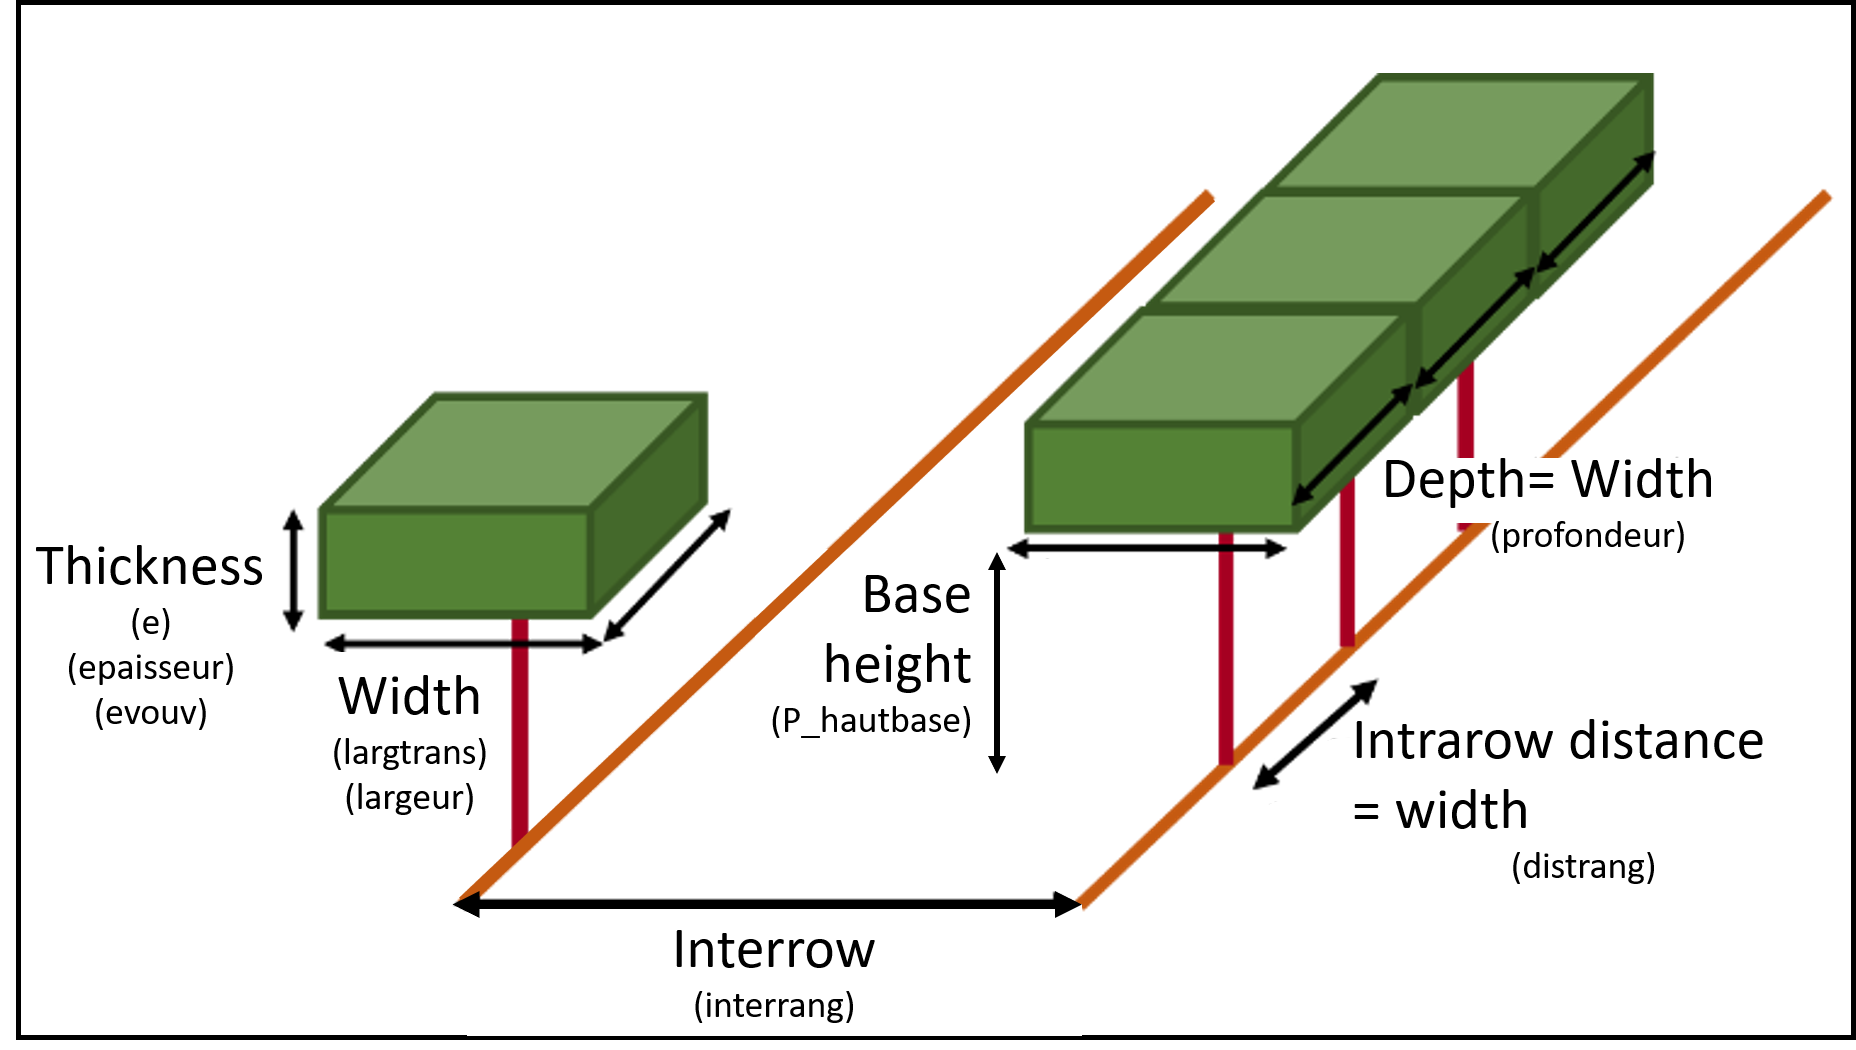
\includegraphics{img/Light-interception-dominant-1.png}
\caption{\label{fig:Width}\textbf{Diagram representing the different
parameters used to compute plant width. The different names used in the
model are shown between parenthesis}}
\end{figure}

\subsection{Plant width correction}\label{plant-width-correction}

If the dominated plant is higher than the base height of the dominant
plant, the radiation interception of the dominant plant is partially
reduced, by reducing the volume that can intercept light to the canopy
volume above the dominated plant only. This correction is made to
consider the competition for light between the two species, and is
computed according to the shape of the plant.

Consequently, the model first compute the height of the dominated plant
(\texttt{sc\%originehaut}) by looking for the maximum height between the
sunlit and shaded part of the dominated plant:\\
\texttt{sc\%originehaut\ =\ max(p(i+1)\%hauteur(sc\%AO),p(i+1)\%hauteur(sc\%AS))}

\begin{quote}
\texttt{sc\%originehaut} is fixed to \texttt{0} (= soil) while computing
the dominated plant.
\end{quote}

Hence, the new thickness (\texttt{enouv}) is computed as:
\(enouv=largeur\cdot\left|varrapforme\right|+hauteurzero\), and is used
to re-compute the shape of the plant:

\begin{itemize}
\tightlist
\item
  The new thickness to width ratio (\texttt{raptrans}, formerly
  \texttt{varrapforme}): \(raptrans=\frac{enouv}{largeur}\) for
  rectangle shaped plants,
\item
  The new width (\texttt{largtrans}, formerly \texttt{largeur}):
  \(largtrans=\frac{enouv}{varrapforme}\) for upsided triangle shaped
  plants,
\item
  The new width (\texttt{largtrans}, formerly \texttt{largeur}):
  \(raptrans=\frac{enouv}{largtrans}\) for downsided triangle shaped
  plants,
\end{itemize}

All variable names are changed, whether there is a correction or not.
Here is a summary table:

\begin{table}

\caption{\label{tab:varmatch}Variable name modification in the formplante function}
\centering
\begin{tabular}[t]{l|l|l}
\hline
Original & Modified & Definition\\
\hline
hauteur & hauteur & Height\\
\hline
largeur & largtrans & Width\\
\hline
varrapforme & raptrans & Thickness/Width Ratio\\
\hline
enouv & enouv & Thickness\\
\hline
\end{tabular}
\end{table}

\begin{quote}
Upside triangle is a triangle with its base at the bottom, while
downside triangle is a triangle with the base at the top.
\end{quote}

The correction of the shape of the plant can be summarised in the
following diagram (\ref{fig:Comprad}):

\begin{figure}
\centering
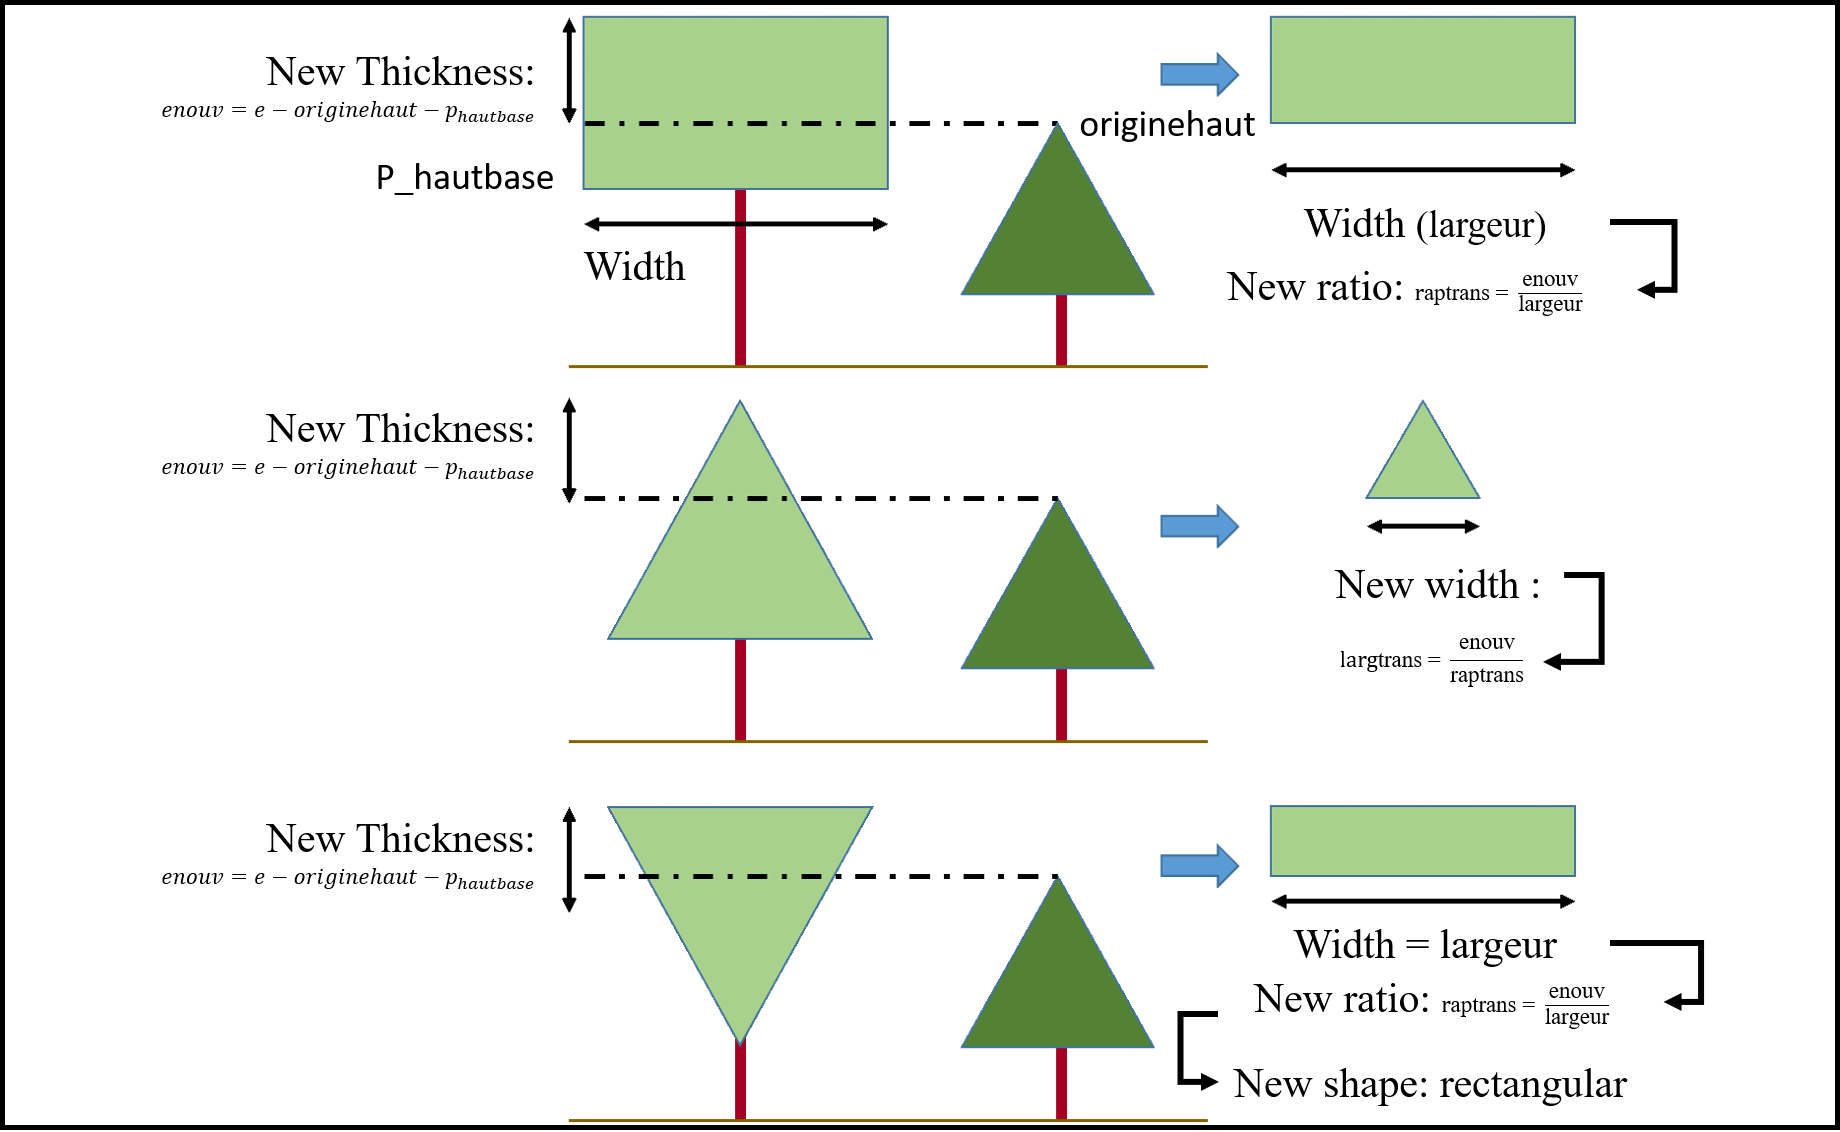
\includegraphics{img/Light-interception-dominant-2.png}
\caption{\label{fig:Comprad}\textbf{Competition for radiation interception
of the dominant plant induced by a high dominated plant}}
\end{figure}

The correction of the shape of the plant is only used to compute the
light transmitted to a plane at the dominated plant or soil height. The
targeted plant interception is computed using its whole leaf area index
and a light extinction coefficient.

\section{Light interception}\label{light-interception}

The light intercepted by a plant species is obtained by computing the
light reaching a horizontal plane below its canopy, either at the height
of the dominated plant (for the dominant plant) of the soil (for the
dominated plant). Therefore, the light incident on this plane is either
coming from:

\begin{itemize}
\tightlist
\item
  The incident light coming from the atmosphere, divided into two
  components, namely the diffuse and direct light. This light is called
  \texttt{rdroit} in the model,
\item
  The light transmitted by the dominant crop, which is called
  \texttt{rtrans}, and that is generally of lower quality for
  photosynthesis. The effect of light quality is wrapped in the
  equivalent density formalism, see \ref{plantdensity} for more details.
\end{itemize}

Consequently, numerous points (20, or 200 if the inter-row is lower than
1 m) are equally distributed every meter along the inter-row
(\emph{i.e.} one point every 5 cm, or every 0.5 cm with 200 points), at
the height of the plane. These points are used to discretize the
computation of the incident light at the surface of the plane.\\
Hence, the total number of points to simulate is computed using the
\texttt{interval} parameter, which is equal to 200 if the inter-row is
lower than 1 meter or 20 if more. It is then used to compute the total
number of points to simulate as:
\(N_{points}=\frac{ir}{2}\cdot interval\)

\begin{quote}
In practice, the model really simulates only half of the inter-row,
because it is considered that the other half have the same light
conditions at daily time-scale. For example, if we take an interrow of
10 meters, the model simulates 100 points equally distributed from 0 to
5 meters.
\end{quote}

Here is an example of the X position on the plane, starting from the
left-hand side of the row, using an inter-row spacing of 1 meter and a
plant width of 0.2 meter:

\begin{Shaded}
\begin{Highlighting}[]
\ControlFlowTok{if}\NormalTok{(ir}\OperatorTok{<}\FloatTok{1.0}\NormalTok{)\{}
\NormalTok{  interval =}\StringTok{ }\DecValTok{200}
\NormalTok{\}}\ControlFlowTok{else}\NormalTok{\{}
\NormalTok{  interval =}\StringTok{ }\DecValTok{20}\NormalTok{.}
\NormalTok{\}}
\NormalTok{i=}\StringTok{ }\DecValTok{1}\OperatorTok{:}\NormalTok{(ir }\OperatorTok{/}\StringTok{ }\DecValTok{2} \OperatorTok{*}\StringTok{ }\NormalTok{interval)}
\NormalTok{x=}\StringTok{ }\NormalTok{(i}\OperatorTok{-}\DecValTok{1}\NormalTok{) }\OperatorTok{/}\StringTok{ }\NormalTok{interval}
\KeywordTok{cat}\NormalTok{(}\KeywordTok{paste}\NormalTok{(}\StringTok{"x="}\NormalTok{, }\KeywordTok{paste}\NormalTok{(x, }\DataTypeTok{collapse =} \StringTok{", "}\NormalTok{)))}
\end{Highlighting}
\end{Shaded}

x= 0, 0.05, 0.1, 0.15, 0.2, 0.25, 0.3, 0.35, 0.4, 0.45

The points are then divided into two groups :

\begin{itemize}
\tightlist
\item
  The sunlit points, which are located directly under the crown of the
  targeted crop.
\item
  The shaded points, which are not directly under the crop crown,
  \emph{i.e.} they have the sky above them.
\end{itemize}

Then the semi-hemisphere above each point is discretized onto 2 x 23
angles: 23 angles from top to right, and 23 angles from top to left.
These angles are used to compute \texttt{kgdiffus}, the atmospheric
diffuse radiation incident to the X point. However, if the X point is
below the targeted crop canopy (\texttt{X\textless{}l/2}), only the 23
angles from the top to the right are used to compute \texttt{kgdiffus}
(considering that Xs are only computed from the left-hand plants row
until the middle of the inter-row, see fig.\ref{fig:Compdominated} for
more details).

The model determines the two angles (\(\theta_1\) and \(\theta_2\))
between which the point only receive incident light coming from the
atmosphere (\texttt{rdroit}). Using these two angles (or their tangent,
\texttt{G}), the model computes:

\begin{enumerate}
\def\labelenumi{\arabic{enumi}.}
\tightlist
\item
  The daily direct radiation (i.e.~cumulated hourly radiation) that is
  incoming only during the time period between two hours (\texttt{h1}
  and \texttt{h2}) when the sun angle is between \(\theta_1\) and
  \(\theta_2\). Function \texttt{kgeom} called in \texttt{rtrans}.
\item
  The incident diffuse radiation for all angles between \(\theta_1\) and
  \(\theta_2\). Function \texttt{kdiff} called in \texttt{rtrans}.
\item
  The light transmitted to the plane by the target crop for all angles
  below \(\theta_1\) or above \(\theta_2\).
\end{enumerate}

\begin{quote}
In practice, all points with an x position lower than
\(\frac{largeur}{2}\) are shaded, and all other are sunlit, so the model
computes the diffuse radiation coming from the atmosphere only for one
quarter of the hemisphere for shaded Xs ; the other quarter will receive
transmitted light because all angles are superior to \(\theta_2\).
\end{quote}

\begin{quote}
Main functions used are \texttt{transrad}, \texttt{rtrans},
\texttt{kdiff} and \texttt{kgeom}.
\end{quote}

The position of \(\theta_1\) and \(\theta_2\) (and their tangent)
depends from three components: the crop shape, its inter-row spacing,
and the sun azimuth (see fig. \ref{fig:Compdominated}).

\begin{figure}
\centering
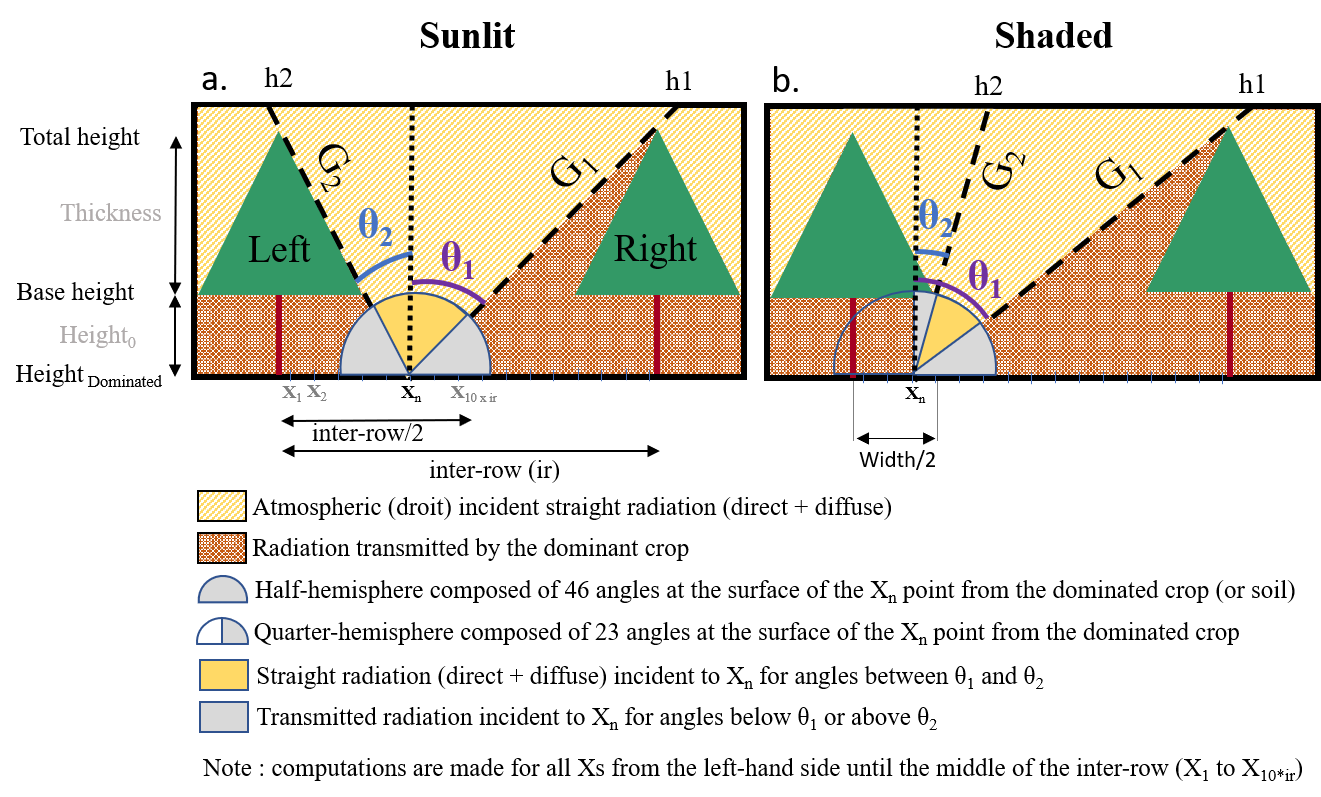
\includegraphics{img/Light-interception-dominated.png}
\caption{\label{fig:Compdominated}\textbf{Diagram of the computation
workflow of STICS for radiation interception for two X points placed
above the dominated plant species. a. The X point is considered sunlit;
b. The X point is considered shaded (right under the dominant plant
canopy), so only the right-hand side of the semi-hemisphere is computed
for atmospheric radiation}}
\end{figure}

\subsection{Incident direct radiation from the
atmosphere}\label{incident-direct-radiation-from-the-atmosphere}

The incident direct radiation for each X point is computed for all
angles of the hemisphere between \(\theta_1\) and \(\theta_2\) (see
\ref{fig:Compdominated}), and summed up to integrate the semi-hemisphere
of each point.

Here is an example of the computation of the direct proportion received
at each X point for a crop. The code is from the \texttt{kgeom()}
function, translated into the R language for compatibility with
\textbf{knitr} (the building machine of this book):

\begin{Shaded}
\begin{Highlighting}[]
\NormalTok{decangle=}\StringTok{ }\ControlFlowTok{function}\NormalTok{(j)\{}
\NormalTok{  theta1 =}\StringTok{ }\DecValTok{2} \OperatorTok{*}\StringTok{ }\NormalTok{pi }\OperatorTok{*}\StringTok{ }\NormalTok{(j }\OperatorTok{-}\StringTok{ }\DecValTok{80}\NormalTok{) }\OperatorTok{/}\StringTok{ }\DecValTok{365}
\NormalTok{  theta2 =}\StringTok{ }\FloatTok{0.034} \OperatorTok{*}\StringTok{ }\NormalTok{(}\KeywordTok{sin}\NormalTok{(}\DecValTok{2} \OperatorTok{*}\StringTok{ }\NormalTok{pi }\OperatorTok{*}\StringTok{ }\NormalTok{j }\OperatorTok{/}\StringTok{ }\DecValTok{365}\NormalTok{) }\OperatorTok{-}\StringTok{ }\KeywordTok{sin}\NormalTok{(}\DecValTok{2} \OperatorTok{*}\StringTok{ }\NormalTok{pi }\OperatorTok{*}\StringTok{ }\DecValTok{80} \OperatorTok{/}\StringTok{ }\DecValTok{365}\NormalTok{))}
\NormalTok{  theta =}\StringTok{ }\NormalTok{theta1 }\OperatorTok{-}\StringTok{ }\NormalTok{theta2}
\NormalTok{  decangle =}\StringTok{ }\KeywordTok{asin}\NormalTok{(}\FloatTok{0.3978} \OperatorTok{*}\StringTok{ }\KeywordTok{sin}\NormalTok{(theta))}
\NormalTok{\}}

\NormalTok{thetacrit=}\StringTok{ }\ControlFlowTok{function}\NormalTok{(lat,j,tgh,alpha)\{}
  
\NormalTok{  acrit =}\StringTok{ }\FloatTok{0.0}
\NormalTok{  bcrit =}\StringTok{ }\FloatTok{0.0}
\NormalTok{  a =}\StringTok{ }\FloatTok{0.0}
\NormalTok{  b =}\StringTok{ }\FloatTok{0.0}
\NormalTok{  thetacr =}\StringTok{ }\FloatTok{0.0}
\NormalTok{  hcritprec=}\StringTok{ }\DecValTok{0}
\NormalTok{  n  =}\StringTok{ }\DecValTok{3}
\NormalTok{  dec =}\StringTok{ }\KeywordTok{decangle}\NormalTok{(j)}
\NormalTok{  hprec =}\StringTok{ }\FloatTok{0.0}
\NormalTok{  pi =}\StringTok{ }\DecValTok{4} \OperatorTok{*}\StringTok{ }\KeywordTok{atan}\NormalTok{(}\FloatTok{1.0}\NormalTok{)}
\NormalTok{  theta=}\StringTok{ }\KeywordTok{rep}\NormalTok{(}\DecValTok{0}\NormalTok{,}\DecValTok{180}\NormalTok{)}
  
  \ControlFlowTok{for}\NormalTok{(i }\ControlFlowTok{in} \DecValTok{1}\OperatorTok{:}\NormalTok{(}\DecValTok{18} \OperatorTok{*}\StringTok{ }\NormalTok{n))\{}
\NormalTok{    theta[i] =}\StringTok{ }\DecValTok{10}\NormalTok{. }\OperatorTok{/}\StringTok{ }\NormalTok{n }\OperatorTok{*}\StringTok{ }\NormalTok{(i }\OperatorTok{-}\StringTok{ }\DecValTok{1}\NormalTok{)}
\NormalTok{    theta[i] =}\StringTok{ }\NormalTok{(theta[i] }\OperatorTok{-}\StringTok{ }\DecValTok{90}\NormalTok{) }\OperatorTok{/}\StringTok{ }\DecValTok{180} \OperatorTok{*}\StringTok{ }\NormalTok{pi}
    \CommentTok{# Sun position (h,azim)}
\NormalTok{    sinh =}\StringTok{ }\KeywordTok{sin}\NormalTok{(lat) }\OperatorTok{*}\StringTok{ }\KeywordTok{sin}\NormalTok{(dec) }\OperatorTok{+}\StringTok{ }\KeywordTok{cos}\NormalTok{(lat) }\OperatorTok{*}\StringTok{ }\KeywordTok{cos}\NormalTok{(dec) }\OperatorTok{*}\StringTok{ }\KeywordTok{cos}\NormalTok{(theta[i])}
\NormalTok{    h =}\StringTok{ }\KeywordTok{asin}\NormalTok{(sinh)}
\NormalTok{    cosazim =}\StringTok{ }\NormalTok{(}\OperatorTok{-}\KeywordTok{cos}\NormalTok{(lat) }\OperatorTok{*}\StringTok{ }\KeywordTok{sin}\NormalTok{(dec) }\OperatorTok{+}\StringTok{ }\KeywordTok{sin}\NormalTok{(lat) }\OperatorTok{*}\StringTok{ }\KeywordTok{cos}\NormalTok{(dec) }\OperatorTok{*}\StringTok{ }\KeywordTok{cos}\NormalTok{(theta[i])) }\OperatorTok{/}\StringTok{ }\KeywordTok{cos}\NormalTok{(h)}
\NormalTok{    cosazim =}\StringTok{ }\KeywordTok{pmin}\NormalTok{(}\FloatTok{1.0}\NormalTok{,cosazim)}
    \ControlFlowTok{if}\NormalTok{(theta[i]}\OperatorTok{!=}\FloatTok{0.0}\NormalTok{)\{}
\NormalTok{      azim =}\StringTok{ }\KeywordTok{acos}\NormalTok{(cosazim) }\OperatorTok{*}\StringTok{ }\NormalTok{theta[i] }\OperatorTok{/}\StringTok{ }\KeywordTok{abs}\NormalTok{(theta[i])}
\NormalTok{    \}}\ControlFlowTok{else}\NormalTok{\{}
\NormalTok{      azim =}\StringTok{ }\FloatTok{0.0}
\NormalTok{    \}}
    \ControlFlowTok{if}\NormalTok{(sinh}\OperatorTok{<}\FloatTok{0.0}\NormalTok{)\{h =}\StringTok{ }\FloatTok{0.0}\NormalTok{\}}
    
    \CommentTok{# Critical height}
\NormalTok{    hcrit =}\StringTok{ }\KeywordTok{atan}\NormalTok{(tgh }\OperatorTok{*}\StringTok{ }\KeywordTok{abs}\NormalTok{(}\KeywordTok{sin}\NormalTok{(azim }\OperatorTok{+}\StringTok{ }\NormalTok{alpha }\OperatorTok{+}\StringTok{ }\FloatTok{0.00001}\NormalTok{)))}
    \CommentTok{# test for h = hcrit}
    \ControlFlowTok{if}\NormalTok{ (hcritprec }\OperatorTok{>=}\StringTok{ }\NormalTok{hprec }\OperatorTok{&}\StringTok{ }\NormalTok{hcrit }\OperatorTok{<=}\StringTok{ }\NormalTok{h }\OperatorTok{&}\StringTok{ }\NormalTok{i }\OperatorTok{>}\StringTok{ }\DecValTok{1}\NormalTok{)\{}
      \CommentTok{# Linear interpolation:}
\NormalTok{      acrit =}\StringTok{ }\NormalTok{(hcrit }\OperatorTok{-}\StringTok{ }\NormalTok{hcritprec) }\OperatorTok{/}\StringTok{ }\NormalTok{(theta[i] }\OperatorTok{-}\StringTok{ }\NormalTok{theta[i}\OperatorTok{-}\DecValTok{1}\NormalTok{])}
\NormalTok{      bcrit =}\StringTok{ }\NormalTok{hcrit }\OperatorTok{-}\StringTok{ }\NormalTok{acrit }\OperatorTok{*}\StringTok{ }\NormalTok{theta[i]}
\NormalTok{      a =}\StringTok{ }\NormalTok{(h }\OperatorTok{-}\StringTok{ }\NormalTok{hprec) }\OperatorTok{/}\StringTok{ }\NormalTok{(theta[i] }\OperatorTok{-}\StringTok{ }\NormalTok{theta[i}\OperatorTok{-}\DecValTok{1}\NormalTok{])}
\NormalTok{      b =}\StringTok{ }\NormalTok{h }\OperatorTok{-}\StringTok{ }\NormalTok{a }\OperatorTok{*}\StringTok{ }\NormalTok{theta[i]}
      
      \ControlFlowTok{if}\NormalTok{(a}\OperatorTok{!=}\NormalTok{acrit)\{thetacr =}\StringTok{ }\NormalTok{(b }\OperatorTok{-}\StringTok{ }\NormalTok{bcrit) }\OperatorTok{/}\StringTok{ }\NormalTok{(acrit }\OperatorTok{-}\StringTok{ }\NormalTok{a)\}}
\NormalTok{      hcritprec =}\StringTok{ }\NormalTok{hcrit}
\NormalTok{      hprec =}\StringTok{ }\NormalTok{h}
\NormalTok{    \}}
\NormalTok{  \}}
  \KeywordTok{return}\NormalTok{(thetacr)}
\NormalTok{\}}

\NormalTok{e =}\StringTok{ }\KeywordTok{abs}\NormalTok{(l }\OperatorTok{*}\StringTok{ }\NormalTok{rap) }\CommentTok{# Thickness of the plant crown}
\NormalTok{xprec=}\StringTok{ }\DecValTok{0}         \CommentTok{# Init.}
\NormalTok{limite =}\StringTok{ }\NormalTok{l }\OperatorTok{/}\StringTok{ }\DecValTok{2}

\ControlFlowTok{if}\NormalTok{(ir}\OperatorTok{<}\FloatTok{1.0}\NormalTok{)\{interval =}\StringTok{ }\DecValTok{200}\NormalTok{.\}}\ControlFlowTok{else}\NormalTok{\{interval =}\StringTok{ }\DecValTok{20}\NormalTok{.\}}
\ControlFlowTok{if}\NormalTok{(l}\OperatorTok{>}\NormalTok{ir}\OperatorTok{/}\DecValTok{2}\NormalTok{.)\{l =}\StringTok{ }\NormalTok{ir}\OperatorTok{/}\DecValTok{2}\NormalTok{.\}}

\ControlFlowTok{if}\NormalTok{(e}\OperatorTok{>}\FloatTok{0.0}\NormalTok{)\{}
\NormalTok{  limite2 =}\StringTok{ }\NormalTok{l}\OperatorTok{/}\DecValTok{2} \OperatorTok{*}\StringTok{ }\NormalTok{(haut}\OperatorTok{/}\NormalTok{e}\OperatorTok{+}\DecValTok{1}\NormalTok{)}
\NormalTok{\}}\ControlFlowTok{else}\NormalTok{\{}
\NormalTok{  P_forme =}\StringTok{ }\DecValTok{1}
\NormalTok{\}}
\CommentTok{# NB : is it sure that it is (haut/e+1) and not (haut/(e+1)) ? }

\CommentTok{# Saving some intermediate results for output here (not in the real function):}
\NormalTok{x_s=}\StringTok{ }\NormalTok{(}\DecValTok{1}\OperatorTok{:}\NormalTok{(ir }\OperatorTok{/}\StringTok{ }\DecValTok{2} \OperatorTok{*}\StringTok{ }\NormalTok{interval))}
\NormalTok{Output=}\StringTok{ }\KeywordTok{data.frame}\NormalTok{(}\DataTypeTok{x_index=}\NormalTok{ x_s,}
                   \DataTypeTok{x_value=}\NormalTok{ (x_s}\OperatorTok{-}\DecValTok{1}\NormalTok{)}\OperatorTok{/}\NormalTok{interval,}
                   \DataTypeTok{theta1=} \KeywordTok{rep}\NormalTok{(}\OtherTok{NA_real_}\NormalTok{,}\KeywordTok{length}\NormalTok{(x_s)),}
                   \DataTypeTok{theta2=} \KeywordTok{rep}\NormalTok{(}\OtherTok{NA_real_}\NormalTok{,}\KeywordTok{length}\NormalTok{(x_s)),}
                   \DataTypeTok{theta1_deg=} \KeywordTok{rep}\NormalTok{(}\OtherTok{NA_real_}\NormalTok{,}\KeywordTok{length}\NormalTok{(x_s)),}
                   \DataTypeTok{theta2_deg=} \KeywordTok{rep}\NormalTok{(}\OtherTok{NA_real_}\NormalTok{,}\KeywordTok{length}\NormalTok{(x_s)),}
                   \DataTypeTok{kg=} \KeywordTok{rep}\NormalTok{(}\DecValTok{0}\NormalTok{,}\KeywordTok{length}\NormalTok{(x_s)))}

\CommentTok{# Loop over Xs:}

\ControlFlowTok{for}\NormalTok{(i }\ControlFlowTok{in}\NormalTok{ x_s)\{}
\NormalTok{  x =}\StringTok{ }\NormalTok{(i}\OperatorTok{-}\DecValTok{1}\NormalTok{) }\OperatorTok{/}\StringTok{ }\NormalTok{interval}
  \ControlFlowTok{if}\NormalTok{(xprec}\OperatorTok{<=}\NormalTok{l}\OperatorTok{/}\DecValTok{2}\OperatorTok{&}\NormalTok{x}\OperatorTok{>=}\NormalTok{l}\OperatorTok{/}\DecValTok{2}\NormalTok{)\{ilim =}\StringTok{ }\NormalTok{i\}}
\NormalTok{  xprec =}\StringTok{ }\NormalTok{x}
  
  \CommentTok{# kdir:}
  
  \CommentTok{# Rectangle:}
  \ControlFlowTok{if}\NormalTok{(P_forme}\OperatorTok{==}\DecValTok{1}\NormalTok{)\{}
\NormalTok{    tgh1 =}\StringTok{ }\NormalTok{(haut }\OperatorTok{+}\StringTok{ }\NormalTok{e) }\OperatorTok{/}\StringTok{ }\NormalTok{(ir }\OperatorTok{-}\StringTok{ }\NormalTok{x }\OperatorTok{-}\StringTok{ }\NormalTok{limite)}
\NormalTok{    theta1 =}\StringTok{ }\KeywordTok{thetacrit}\NormalTok{(lat,j,tgh1,alpha)}
    \ControlFlowTok{if}\NormalTok{(x}\OperatorTok{>}\NormalTok{limite)\{}
\NormalTok{      tgh2 =}\StringTok{ }\NormalTok{(haut }\OperatorTok{+}\StringTok{ }\NormalTok{e) }\OperatorTok{/}\StringTok{ }\NormalTok{(x }\OperatorTok{-}\StringTok{ }\NormalTok{limite)}
\NormalTok{      theta2 =}\StringTok{ }\KeywordTok{thetacrit}\NormalTok{(lat,j,tgh2,alpha)}
\NormalTok{    \}}\ControlFlowTok{else} \ControlFlowTok{if}\NormalTok{(x }\OperatorTok{<}\StringTok{ }\NormalTok{limite)\{}
\NormalTok{      tgh2 =}\StringTok{ }\NormalTok{haut }\OperatorTok{/}\StringTok{ }\NormalTok{( }\OperatorTok{-}\NormalTok{x }\OperatorTok{+}\StringTok{ }\NormalTok{limite)}
\NormalTok{      theta2 =}\StringTok{ }\OperatorTok{-}\KeywordTok{thetacrit}\NormalTok{(lat,j,tgh2,alpha)}
\NormalTok{    \}}\ControlFlowTok{else}\NormalTok{\{}
      \CommentTok{# x == limite}
\NormalTok{      theta2 =}\StringTok{ }\DecValTok{0}
\NormalTok{    \}}
\NormalTok{  \}}
  
  \CommentTok{# Downside Triangle:}
  \ControlFlowTok{if}\NormalTok{ (P_forme}\OperatorTok{==}\DecValTok{2} \OperatorTok{&}\StringTok{ }\NormalTok{rap}\OperatorTok{<}\DecValTok{0}\NormalTok{.)\{}
\NormalTok{    tgh1 =}\StringTok{ }\NormalTok{(haut }\OperatorTok{+}\StringTok{ }\NormalTok{e) }\OperatorTok{/}\StringTok{ }\NormalTok{(ir }\OperatorTok{-}\StringTok{ }\NormalTok{x }\OperatorTok{-}\StringTok{ }\NormalTok{limite)}
\NormalTok{    theta1 =}\StringTok{ }\KeywordTok{thetacrit}\NormalTok{(lat,j,tgh1,alpha)}
    \ControlFlowTok{if}\NormalTok{ (x }\OperatorTok{>}\StringTok{ }\NormalTok{limite)\{}
\NormalTok{      tgh2 =}\StringTok{ }\NormalTok{(haut }\OperatorTok{+}\StringTok{ }\NormalTok{e) }\OperatorTok{/}\StringTok{ }\NormalTok{(x }\OperatorTok{-}\StringTok{ }\NormalTok{limite)}
\NormalTok{      theta2 =}\StringTok{ }\KeywordTok{thetacrit}\NormalTok{(lat,j,tgh2,alpha)}
\NormalTok{    \}}\ControlFlowTok{else} \ControlFlowTok{if}\NormalTok{(x }\OperatorTok{<}\StringTok{ }\NormalTok{limite)\{}
\NormalTok{      tgh2 =}\StringTok{ }\NormalTok{(haut }\OperatorTok{+}\StringTok{ }\NormalTok{e) }\OperatorTok{/}\StringTok{ }\NormalTok{( x }\OperatorTok{-}\StringTok{ }\NormalTok{limite)}
\NormalTok{      theta2 =}\StringTok{ }\OperatorTok{-}\KeywordTok{thetacrit}\NormalTok{(lat,j,tgh2,alpha)}
\NormalTok{    \}}\ControlFlowTok{else}\NormalTok{\{}
\NormalTok{      theta2 =}\StringTok{ }\DecValTok{0}
\NormalTok{    \}}
\NormalTok{  \}}
  
  \CommentTok{# Upside Triangle:}
  \ControlFlowTok{if}\NormalTok{ (P_forme}\OperatorTok{==}\DecValTok{2}\OperatorTok{&}\NormalTok{rap}\OperatorTok{>}\DecValTok{0}\NormalTok{.)\{ then}
\NormalTok{    tgh1 =}\StringTok{ }\NormalTok{(haut }\OperatorTok{+}\StringTok{ }\NormalTok{e) }\OperatorTok{/}\StringTok{ }\NormalTok{(ir }\OperatorTok{-}\StringTok{ }\NormalTok{x }\OperatorTok{-}\StringTok{ }\NormalTok{limite)}
\NormalTok{    theta1 =}\StringTok{ }\KeywordTok{thetacrit}\NormalTok{(lat,j,tgh1,alpha)}
    \ControlFlowTok{if}\NormalTok{ (x }\OperatorTok{<}\StringTok{ }\NormalTok{limite2)\{}
      \ControlFlowTok{if}\NormalTok{ (x }\OperatorTok{>}\StringTok{ }\NormalTok{limite)\{}
\NormalTok{        tgh2 =}\StringTok{ }\NormalTok{haut }\OperatorTok{/}\StringTok{ }\NormalTok{( x }\OperatorTok{-}\StringTok{ }\NormalTok{limite)}
\NormalTok{        theta2 =}\StringTok{ }\KeywordTok{thetacrit}\NormalTok{(lat,j,tgh2,alpha)}
\NormalTok{      \}}\ControlFlowTok{else} \ControlFlowTok{if}\NormalTok{(x }\OperatorTok{<}\StringTok{ }\NormalTok{limite)\{}
\NormalTok{        tgh2 =}\StringTok{ }\NormalTok{haut }\OperatorTok{/}\StringTok{ }\NormalTok{(limite }\OperatorTok{-}\StringTok{ }\NormalTok{x)}
\NormalTok{        theta2 =}\StringTok{ }\OperatorTok{-}\KeywordTok{thetacrit}\NormalTok{(lat,j,tgh2,alpha)}
\NormalTok{      \}}\ControlFlowTok{else}\NormalTok{\{}
\NormalTok{        theta2 =}\StringTok{ }\FloatTok{0.0}
\NormalTok{      \}}
\NormalTok{    \}}\ControlFlowTok{else} \ControlFlowTok{if}\NormalTok{(x }\OperatorTok{>=}\StringTok{ }\NormalTok{limite2)\{}
\NormalTok{      tgh2 =}\StringTok{ }\NormalTok{(haut }\OperatorTok{+}\StringTok{ }\NormalTok{e) }\OperatorTok{/}\StringTok{ }\NormalTok{x}
\NormalTok{      theta2 =}\StringTok{ }\KeywordTok{thetacrit}\NormalTok{(lat,j,tgh2,alpha)}
\NormalTok{    \}}
\NormalTok{  \}}
  
  \CommentTok{# NB: is there a missing else here ? kg is modified just after...}
  \ControlFlowTok{if}\NormalTok{(e }\OperatorTok{>}\StringTok{ }\FloatTok{2.1e-2}\NormalTok{)\{}
\NormalTok{    kg =}\StringTok{ }\KeywordTok{cos}\NormalTok{(theta1)}
\NormalTok{    kg =}\StringTok{ }\KeywordTok{cos}\NormalTok{(theta2)}
\NormalTok{  \}}
\NormalTok{  kg =}\StringTok{ }\FloatTok{0.5} \OperatorTok{*}\StringTok{ }\NormalTok{(}\KeywordTok{cos}\NormalTok{(pi}\OperatorTok{/}\DecValTok{2} \OperatorTok{+}\StringTok{ }\NormalTok{theta1) }\OperatorTok{+}\StringTok{ }\KeywordTok{cos}\NormalTok{(pi}\OperatorTok{/}\DecValTok{2} \OperatorTok{+}\StringTok{ }\NormalTok{theta2))}
\NormalTok{  kg =}\StringTok{ }\KeywordTok{max}\NormalTok{(kg,}\FloatTok{0.0}\NormalTok{)}
  
\NormalTok{  Output}\OperatorTok{$}\NormalTok{theta1[Output}\OperatorTok{$}\NormalTok{x_index}\OperatorTok{==}\NormalTok{i]=}\StringTok{ }\NormalTok{theta1}
\NormalTok{  Output}\OperatorTok{$}\NormalTok{theta2[Output}\OperatorTok{$}\NormalTok{x_index}\OperatorTok{==}\NormalTok{i]=}\StringTok{ }\NormalTok{theta2}
\NormalTok{  Output}\OperatorTok{$}\NormalTok{kg[Output}\OperatorTok{$}\NormalTok{x_index}\OperatorTok{==}\NormalTok{i]=}\StringTok{ }\NormalTok{kg}
\NormalTok{\}}

\NormalTok{Output}\OperatorTok{$}\NormalTok{theta1_deg=}\StringTok{ }\NormalTok{(pi}\OperatorTok{/}\DecValTok{2}\OperatorTok{+}\NormalTok{Output}\OperatorTok{$}\NormalTok{theta1)}\OperatorTok{*}\DecValTok{180}\OperatorTok{/}\NormalTok{pi}
\NormalTok{Output}\OperatorTok{$}\NormalTok{theta2_deg=}\StringTok{ }\NormalTok{(pi}\OperatorTok{/}\DecValTok{2}\OperatorTok{-}\NormalTok{Output}\OperatorTok{$}\NormalTok{theta2)}\OperatorTok{*}\DecValTok{180}\OperatorTok{/}\NormalTok{pi}

\KeywordTok{colnames}\NormalTok{(Output)=}\StringTok{ }\KeywordTok{c}\NormalTok{(}\StringTok{"X index"}\NormalTok{,}\StringTok{"X value (m)"}\NormalTok{,}\StringTok{"Theta 1 (rad)"}\NormalTok{,}\StringTok{"Theta 2 (rad)"}\NormalTok{,}
                    \StringTok{"Theta 1 (deg)"}\NormalTok{,}\StringTok{"Theta 2 (deg)"}\NormalTok{,}\StringTok{"kgdirect"}\NormalTok{)}

\KeywordTok{kable}\NormalTok{(Output, }\DataTypeTok{caption=} \KeywordTok{paste}\NormalTok{(}\StringTok{"Example of the computation of the incident direct"}\NormalTok{,}
                             \StringTok{"radiation ratio kgdirect. See introduction section"}\NormalTok{,}
                             \StringTok{"for further details on the crop."}\NormalTok{))}
\end{Highlighting}
\end{Shaded}

\begin{table}

\caption{\label{tab:kdir}Example of the computation of the incident direct radiation ratio kgdirect. See introduction section for further details on the crop.}
\centering
\begin{tabular}[t]{r|r|r|r|r|r|r}
\hline
X index & X value (m) & Theta 1 (rad) & Theta 2 (rad) & Theta 1 (deg) & Theta 2 (deg) & kgdirect\\
\hline
1 & 0.00 & -0.7563093 & 0.1163553 & 46.66667 & 83.33333 & 0.2850744\\
\hline
2 & 0.05 & -0.7563093 & 0.0581776 & 46.66667 & 86.66667 & 0.3140484\\
\hline
3 & 0.10 & -0.6981317 & 0.0000000 & 50.00000 & 90.00000 & 0.3213938\\
\hline
4 & 0.15 & -0.6981317 & -0.0581776 & 50.00000 & 93.33333 & 0.3504662\\
\hline
5 & 0.20 & -0.6399541 & -0.1163553 & 53.33333 & 96.66667 & 0.3566258\\
\hline
6 & 0.25 & -0.6399541 & -0.1745329 & 53.33333 & 100.00000 & 0.3854034\\
\hline
7 & 0.30 & -0.5817764 & -0.2327106 & 56.66667 & 103.33333 & 0.3900624\\
\hline
8 & 0.35 & -0.5235988 & -0.2908882 & 60.00000 & 106.66667 & 0.3934016\\
\hline
9 & 0.40 & -0.4654211 & -0.2908882 & 63.33333 & 106.66667 & 0.3678012\\
\hline
10 & 0.45 & -0.4654211 & -0.3490659 & 63.33333 & 110.00000 & 0.3954097\\
\hline
\end{tabular}
\end{table}

Where \(\theta_1\) and \(\theta_2\) are the angles visible in
\protect\hyperlink{fig:Compdominated}{fig.3} and kgdirect the proportion
of the semi-hemisphere that receive direct light, considering sun
position throughout the day by using stand latitude, day of year and row
orientation. In the model, \(\theta_1\) and \(\theta_2\) are computed in
radian relative to the vertical plane above X. To provide a simpler
representation, \(\theta_1\) and \(\theta_2\) are also given in degrees
relative to the horizontal plane (i.e.~soil or dominated plant species
surface) in tab.\ref{tab:kdir}.

\subsection{Incident diffuse radiation from the
atmosphere}\label{incident-diffuse-radiation-from-the-atmosphere}

The incident diffuse radiation for all angles between \(\theta_1\) and
\(\theta_2\) is computed using \texttt{G}, the apparent tangent to the
considered \(\theta\). First the model computes it for \(\theta_1\), and
uses it as a threshold under which no diffuse radiation comes from the
atmosphere because only transmitted radiation reaches this angle for the
considered X point. Second, the model tests if the X point is below the
target crop canopy, and if not it computes \texttt{G} for \(\theta_2\),
and applies the same methodology, with \texttt{G} being the upper
threshold this time. This method avoids computing the left-hand quarter
of the hemisphere since it receives only transmitted light necessarily
if it is under the targeted crop.

Here is an example of the computation of the diffuse proportion received
at each X point for the same crop as above (interrow= 1 meter, width=
0.2 meter, thickness= 0.1 meter, height= 1 meter). The code is from the
\texttt{kdif()} function, translated into R:

\begin{Shaded}
\begin{Highlighting}[]
\CommentTok{# Initializations:}
\NormalTok{htab=}\StringTok{ }\KeywordTok{c}\NormalTok{(}\FloatTok{9.23}\NormalTok{, }\FloatTok{9.23}\NormalTok{, }\FloatTok{9.23}\NormalTok{, }\FloatTok{9.23}\NormalTok{, }\FloatTok{9.23}\NormalTok{, }\FloatTok{10.81}\NormalTok{, }\FloatTok{10.81}\NormalTok{, }\FloatTok{26.57}\NormalTok{,}
        \FloatTok{26.57}\NormalTok{, }\FloatTok{26.57}\NormalTok{, }\FloatTok{31.08}\NormalTok{, }\FloatTok{31.08}\NormalTok{, }\FloatTok{31.08}\NormalTok{, }\FloatTok{31.08}\NormalTok{, }\FloatTok{31.08}\NormalTok{, }\FloatTok{47.41}\NormalTok{,}
        \FloatTok{47.41}\NormalTok{, }\FloatTok{47.41}\NormalTok{, }\FloatTok{52.62}\NormalTok{, }\FloatTok{52.62}\NormalTok{, }\FloatTok{69.16}\NormalTok{, }\FloatTok{69.16}\NormalTok{, }\FloatTok{69.16}\NormalTok{)}
\NormalTok{aztab=}\StringTok{ }\KeywordTok{c}\NormalTok{(}\FloatTok{12.23}\NormalTok{,}\FloatTok{59.77}\NormalTok{,}\FloatTok{84.23}\NormalTok{,}\FloatTok{131.77}\NormalTok{,}\FloatTok{156.23}\NormalTok{,}\DecValTok{36}\NormalTok{,}\DecValTok{108}\NormalTok{,}\DecValTok{0}\NormalTok{,}\DecValTok{72}\NormalTok{,}\DecValTok{144}\NormalTok{,}\FloatTok{23.27}\NormalTok{,}\FloatTok{48.73}\NormalTok{,}\FloatTok{95.27}\NormalTok{,}
         \FloatTok{120.73}\NormalTok{,}\FloatTok{167.27}\NormalTok{,}\DecValTok{0}\NormalTok{,}\DecValTok{72}\NormalTok{,}\DecValTok{144}\NormalTok{,}\DecValTok{36}\NormalTok{,}\DecValTok{108}\NormalTok{,}\DecValTok{0}\NormalTok{,}\DecValTok{72}\NormalTok{,}\DecValTok{144}\NormalTok{)}
\NormalTok{SOCtab=}\StringTok{ }\KeywordTok{c}\NormalTok{(}\FloatTok{0.0043}\NormalTok{, }\FloatTok{0.0043}\NormalTok{, }\FloatTok{0.0043}\NormalTok{, }\FloatTok{0.0043}\NormalTok{, }\FloatTok{0.0043}\NormalTok{, }\FloatTok{0.0055}\NormalTok{,}
          \FloatTok{0.0055}\NormalTok{, }\FloatTok{0.0140}\NormalTok{, }\FloatTok{0.0140}\NormalTok{, }\FloatTok{0.0140}\NormalTok{, }\FloatTok{0.0197}\NormalTok{, }\FloatTok{0.0197}\NormalTok{,}
          \FloatTok{0.0197}\NormalTok{, }\FloatTok{0.0197}\NormalTok{, }\FloatTok{0.0197}\NormalTok{, }\FloatTok{0.0336}\NormalTok{, }\FloatTok{0.0336}\NormalTok{, }\FloatTok{0.0336}\NormalTok{,}
          \FloatTok{0.0399}\NormalTok{, }\FloatTok{0.0399}\NormalTok{, }\FloatTok{0.0495}\NormalTok{, }\FloatTok{0.0495}\NormalTok{, }\FloatTok{0.0495}\NormalTok{)}
\NormalTok{xprec=}\StringTok{ }\DecValTok{0}

\ControlFlowTok{if}\NormalTok{(ir}\OperatorTok{<}\FloatTok{1.0}\NormalTok{)\{interval =}\StringTok{ }\DecValTok{200}\NormalTok{.\}}\ControlFlowTok{else}\NormalTok{\{interval =}\StringTok{ }\DecValTok{20}\NormalTok{.\}}
\ControlFlowTok{if}\NormalTok{(l}\OperatorTok{>}\NormalTok{ir}\OperatorTok{/}\DecValTok{2}\NormalTok{.)\{l =}\StringTok{ }\NormalTok{ir}\OperatorTok{/}\DecValTok{2}\NormalTok{.\}}

\CommentTok{# Saving some intermediate results for Output_diff here (not in the real function):}
\NormalTok{x_s=}\StringTok{ }\NormalTok{(}\DecValTok{1}\OperatorTok{:}\NormalTok{(ir }\OperatorTok{/}\StringTok{ }\DecValTok{2} \OperatorTok{*}\StringTok{ }\NormalTok{interval))}
\NormalTok{Output_diff=}\StringTok{ }\KeywordTok{data.frame}\NormalTok{(}\DataTypeTok{x_index=} \KeywordTok{rep}\NormalTok{(x_s,}\DataTypeTok{each=}\DecValTok{23}\NormalTok{),}
                   \DataTypeTok{x_value=} \KeywordTok{rep}\NormalTok{((x_s}\OperatorTok{-}\DecValTok{1}\NormalTok{)}\OperatorTok{/}\NormalTok{interval,}\DataTypeTok{each=}\DecValTok{23}\NormalTok{),}
                   \DataTypeTok{Angle =} \KeywordTok{rep}\NormalTok{(}\DecValTok{1}\OperatorTok{:}\DecValTok{23}\NormalTok{, }\KeywordTok{length}\NormalTok{(x_s)),}
                   \DataTypeTok{G1=} \KeywordTok{rep}\NormalTok{(}\OtherTok{NA_real_}\NormalTok{,}\KeywordTok{length}\NormalTok{(x_s)}\OperatorTok{*}\DecValTok{23}\NormalTok{),}
                   \DataTypeTok{G2=} \KeywordTok{rep}\NormalTok{(}\OtherTok{NA_real_}\NormalTok{,}\KeywordTok{length}\NormalTok{(x_s)}\OperatorTok{*}\DecValTok{23}\NormalTok{),}
                   \DataTypeTok{hcrit=} \KeywordTok{rep}\NormalTok{(}\DecValTok{0}\NormalTok{,}\KeywordTok{length}\NormalTok{(x_s)}\OperatorTok{*}\DecValTok{23}\NormalTok{),}
                   \DataTypeTok{kgdiffus=} \KeywordTok{rep}\NormalTok{(}\DecValTok{0}\NormalTok{,}\KeywordTok{length}\NormalTok{(x_s)}\OperatorTok{*}\DecValTok{23}\NormalTok{))}


\CommentTok{# Loop over Xs:}

\ControlFlowTok{for}\NormalTok{(i }\ControlFlowTok{in}\NormalTok{ x_s)\{}
\NormalTok{  x =}\StringTok{ }\NormalTok{(i}\OperatorTok{-}\DecValTok{1}\NormalTok{) }\OperatorTok{/}\StringTok{ }\NormalTok{interval}
  \ControlFlowTok{if}\NormalTok{(xprec}\OperatorTok{<=}\NormalTok{l}\OperatorTok{/}\DecValTok{2}\OperatorTok{&}\NormalTok{x}\OperatorTok{>=}\NormalTok{l}\OperatorTok{/}\DecValTok{2}\NormalTok{)\{ilim =}\StringTok{ }\NormalTok{i\}}
\NormalTok{  xprec =}\StringTok{ }\NormalTok{x}
  
  \CommentTok{# kdif:}
  
\NormalTok{  x =}\StringTok{ }\KeywordTok{min}\NormalTok{(x,ir}\OperatorTok{/}\DecValTok{2}\NormalTok{)}
\NormalTok{  e =}\StringTok{ }\KeywordTok{abs}\NormalTok{(l}\OperatorTok{*}\NormalTok{rap)}
\NormalTok{  kgdiffus =}\StringTok{ }\DecValTok{0}\NormalTok{.}
  
  \CommentTok{# Computing for the right-hand of the row:}
\NormalTok{  G1 =}\StringTok{ }\NormalTok{(haut}\OperatorTok{+}\NormalTok{e)}\OperatorTok{/}\NormalTok{(ir}\OperatorTok{-}\NormalTok{x}\OperatorTok{-}\NormalTok{l}\OperatorTok{/}\DecValTok{2}\NormalTok{.) }\CommentTok{# the apparent tangent h1}
  \ControlFlowTok{for}\NormalTok{(j }\ControlFlowTok{in} \DecValTok{1}\OperatorTok{:}\DecValTok{23}\NormalTok{)\{}
\NormalTok{    hcrit =}\StringTok{ }\KeywordTok{atan}\NormalTok{(G1}\OperatorTok{*}\KeywordTok{sin}\NormalTok{(aztab[j]}\OperatorTok{/}\DecValTok{180}\OperatorTok{*}\NormalTok{pi))}\OperatorTok{/}\NormalTok{pi}\OperatorTok{*}\DecValTok{180}
    \ControlFlowTok{if}\NormalTok{(hcrit}\OperatorTok{<}\NormalTok{htab[j])\{}
\NormalTok{      kgdiffus =}\StringTok{ }\NormalTok{kgdiffus}\OperatorTok{+}\NormalTok{SOCtab[j]}
\NormalTok{      ######## Not in the real function ########}
\NormalTok{      Output_diff}\OperatorTok{$}\NormalTok{kgdiffus[Output_diff}\OperatorTok{$}\NormalTok{x_index}\OperatorTok{==}\NormalTok{i}\OperatorTok{&}\NormalTok{Output_diff}\OperatorTok{$}\NormalTok{Angle}\OperatorTok{==}\NormalTok{j]=}\StringTok{ }\NormalTok{SOCtab[j]}
\NormalTok{      ##########################################}
\NormalTok{    \}}
\NormalTok{    ######## Not in the real function ########}
\NormalTok{    Output_diff}\OperatorTok{$}\NormalTok{hcrit[Output_diff}\OperatorTok{$}\NormalTok{x_index}\OperatorTok{==}\NormalTok{i}\OperatorTok{&}\NormalTok{Output_diff}\OperatorTok{$}\NormalTok{Angle}\OperatorTok{==}\NormalTok{j]=}\StringTok{ }\NormalTok{hcrit}
\NormalTok{    Output_diff}\OperatorTok{$}\NormalTok{G1[Output_diff}\OperatorTok{$}\NormalTok{x_index}\OperatorTok{==}\NormalTok{i}\OperatorTok{&}\NormalTok{Output_diff}\OperatorTok{$}\NormalTok{Angle}\OperatorTok{==}\NormalTok{j]=}\StringTok{ }\NormalTok{G1}
\NormalTok{    ##########################################}
\NormalTok{  \}}
  
  \CommentTok{# Computing for the left-hand row, if the point is not a shaded point:}
  \ControlFlowTok{if}\NormalTok{(x}\OperatorTok{>}\NormalTok{l}\OperatorTok{/}\DecValTok{2}\NormalTok{)\{}
\NormalTok{    G2 =}\StringTok{ }\NormalTok{(haut}\OperatorTok{+}\NormalTok{e)}\OperatorTok{/}\NormalTok{(x}\OperatorTok{-}\NormalTok{l}\OperatorTok{/}\DecValTok{2}\NormalTok{) }\CommentTok{# the apparent tangent h2}
    \ControlFlowTok{for}\NormalTok{(j }\ControlFlowTok{in} \DecValTok{1}\OperatorTok{:}\DecValTok{23}\NormalTok{)\{}
\NormalTok{      hcrit =}\StringTok{ }\KeywordTok{atan}\NormalTok{(G2}\OperatorTok{*}\KeywordTok{sin}\NormalTok{(aztab[j]}\OperatorTok{/}\DecValTok{180}\OperatorTok{*}\NormalTok{pi))}\OperatorTok{/}\NormalTok{pi}\OperatorTok{*}\DecValTok{180}
      \ControlFlowTok{if}\NormalTok{(hcrit }\OperatorTok{<}\StringTok{ }\NormalTok{htab[j])\{}
\NormalTok{        kgdiffus =}\StringTok{ }\NormalTok{kgdiffus}\OperatorTok{+}\NormalTok{SOCtab[j]}
\NormalTok{        ######## Not in the real function ########}
\NormalTok{        Output_diff}\OperatorTok{$}\NormalTok{kgdiffus[Output_diff}\OperatorTok{$}\NormalTok{x_index}\OperatorTok{==}\NormalTok{i}\OperatorTok{&}\NormalTok{Output_diff}\OperatorTok{$}\NormalTok{Angle}\OperatorTok{==}\NormalTok{j]=}\StringTok{ }
\StringTok{          }\NormalTok{Output_diff}\OperatorTok{$}\NormalTok{kgdiffus[Output_diff}\OperatorTok{$}\NormalTok{x_index}\OperatorTok{==}\NormalTok{i}\OperatorTok{&}\NormalTok{Output_diff}\OperatorTok{$}\NormalTok{Angle}\OperatorTok{==}\NormalTok{j]}\OperatorTok{+}\NormalTok{SOCtab[j]}
\NormalTok{        ##########################################}
\NormalTok{      \}}
\NormalTok{      ######## Not in the real function ########}
\NormalTok{      Output_diff}\OperatorTok{$}\NormalTok{hcrit[Output_diff}\OperatorTok{$}\NormalTok{x_index}\OperatorTok{==}\NormalTok{i}\OperatorTok{&}\NormalTok{Output_diff}\OperatorTok{$}\NormalTok{Angle}\OperatorTok{==}\NormalTok{j]=}\StringTok{ }\NormalTok{hcrit}
\NormalTok{      Output_diff}\OperatorTok{$}\NormalTok{G2[Output_diff}\OperatorTok{$}\NormalTok{x_index}\OperatorTok{==}\NormalTok{i}\OperatorTok{&}\NormalTok{Output_diff}\OperatorTok{$}\NormalTok{Angle}\OperatorTok{==}\NormalTok{j]=}\StringTok{ }\NormalTok{G2}
\NormalTok{      ##########################################}
\NormalTok{    \}}
\NormalTok{  \}}
\NormalTok{\}}

\KeywordTok{colnames}\NormalTok{(Output_diff)=}\StringTok{ }\KeywordTok{c}\NormalTok{(}\StringTok{"X index"}\NormalTok{,}\StringTok{"X value (m)"}\NormalTok{,}\StringTok{"angle"}\NormalTok{,}\StringTok{"G1 (tangent)"}\NormalTok{,}
                         \StringTok{"G2 (tangent)"}\NormalTok{,}\StringTok{"hcrit"}\NormalTok{,}\StringTok{"kgdiffus"}\NormalTok{)}
\ControlFlowTok{if}\NormalTok{(knitr}\OperatorTok{:::}\KeywordTok{pandoc_to}\NormalTok{() }\OperatorTok{==}\StringTok{ "html"}\NormalTok{) \{Output_diff\}}\ControlFlowTok{else}\NormalTok{\{}
  \KeywordTok{kable}\NormalTok{(Output_diff[}\DecValTok{1}\OperatorTok{:}\DecValTok{10}\NormalTok{,],}
        \DataTypeTok{caption =} \KeywordTok{paste}\NormalTok{(}\StringTok{"Computation of the diffuse light incident on each"}\NormalTok{,}
                        \StringTok{"point x. Ten first rows only, for the full data,"}\NormalTok{,}
                        \StringTok{"please refer to the html version of this book"}\NormalTok{),}
        \DataTypeTok{col.names =} \KeywordTok{c}\NormalTok{(}\StringTok{"X index"}\NormalTok{,}\StringTok{"X value (m)"}\NormalTok{,}\StringTok{"angle"}\NormalTok{,}\StringTok{"G1 (tangent)"}\NormalTok{,}
                      \StringTok{"G2 (tangent)"}\NormalTok{,}\StringTok{"hcrit"}\NormalTok{,}\StringTok{"kgdiffus"}\NormalTok{), }\DataTypeTok{longtable =} \OtherTok{TRUE}\NormalTok{)}
\NormalTok{\}}
\end{Highlighting}
\end{Shaded}

\begin{longtable}[t]{r|r|r|r|r|r|r}
\caption{\label{tab:kdiff}Computation of the diffuse light incident on each point x. Ten first rows only, for the full data, please refer to the html version of this book}\\
\hline
X index & X value (m) & angle & G1 (tangent) & G2 (tangent) & hcrit & kgdiffus\\
\hline
1 & 0 & 1 & 1.222222 & NA & 14.51577 & 0.000\\
\hline
1 & 0 & 2 & 1.222222 & NA & 46.56057 & 0.000\\
\hline
1 & 0 & 3 & 1.222222 & NA & 50.56789 & 0.000\\
\hline
1 & 0 & 4 & 1.222222 & NA & 42.35117 & 0.000\\
\hline
1 & 0 & 5 & 1.222222 & NA & 26.22654 & 0.000\\
\hline
1 & 0 & 6 & 1.222222 & NA & 35.69363 & 0.000\\
\hline
1 & 0 & 7 & 1.222222 & NA & 49.29501 & 0.000\\
\hline
1 & 0 & 8 & 1.222222 & NA & 0.00000 & 0.014\\
\hline
1 & 0 & 9 & 1.222222 & NA & 49.29501 & 0.000\\
\hline
1 & 0 & 10 & 1.222222 & NA & 35.69363 & 0.000\\
\hline
\end{longtable}

The total diffuse radiation incident to each point X is simply the
cumulative of each angle:

\begin{Shaded}
\begin{Highlighting}[]
\KeywordTok{suppressWarnings}\NormalTok{(}\KeywordTok{suppressPackageStartupMessages}\NormalTok{(}\KeywordTok{library}\NormalTok{(dplyr)))}
\NormalTok{Output_diff}\OperatorTok
\StringTok{  }\KeywordTok{group_by}\NormalTok{(}\StringTok{`}\DataTypeTok{X index}\StringTok{`}\NormalTok{)}\OperatorTok
\StringTok{  }\KeywordTok{summarise}\NormalTok{(}\DataTypeTok{kgdiffus=} \KeywordTok{sum}\NormalTok{(kgdiffus))}

\KeywordTok{kable}\NormalTok{(Output_diff,}\DataTypeTok{caption=} \KeywordTok{paste}\NormalTok{(}\StringTok{"Example of the computation of the incident diffuse"}\NormalTok{,}
\StringTok{"radiation ratio kgdiffus. See introduction section for further details on the crop."}\NormalTok{))}
\end{Highlighting}
\end{Shaded}

\begin{table}

\caption{\label{tab:kdifftot}Example of the computation of the incident diffuse radiation ratio kgdiffus. See introduction section for further details on the crop.}
\centering
\begin{tabular}[t]{r|r}
\hline
X index & kgdiffus\\
\hline
1 & 0.3489\\
\hline
2 & 0.3489\\
\hline
3 & 0.3489\\
\hline
4 & 0.4061\\
\hline
5 & 0.3864\\
\hline
6 & 0.3864\\
\hline
7 & 0.3864\\
\hline
8 & 0.4023\\
\hline
9 & 0.4023\\
\hline
10 & 0.3624\\
\hline
\end{tabular}
\end{table}

\subsection{Total diffuse and direct radiation from the atmosphere
incident to each X
point}\label{total-diffuse-and-direct-radiation-from-the-atmosphere-incident-to-each-x-point}

The total radiation from the atmosphere incident to each X point is
computed by using the incident diffuse (\texttt{rdif}) and direct
(\texttt{rdirect}) radiation coming from the atmosphere weighted
respectively by the previously computed \texttt{kgdiffus} and
\texttt{kgdirect} as follow:
\(rdroit=(kgdiffus\cdot rdif)+(kgdirect\cdot rdirect)\)

\subsection{Light tramsitted by the dominant crop to the X
points}\label{light-tramsitted-by-the-dominant-crop-to-the-x-points}

The light transmitted by the dominant crop to the dominated crop
(\texttt{rtransmis}) is computed using the total radiation from the
atmosphere incident to each X point (\texttt{rdroit}) and the effective
targeted plant leaf area index as follow:

\(rtransmis=(1.0-rdroit)\cdot e^{-P_{ktrou}\cdot(lai+eai)}\)

where \(P_{ktrou}\) is the targeted plant light extinction coefficient,
\texttt{lai} the plant leaf area index, and \texttt{eai} the equivalent
leaf area index, which represent the photosynthetic surface that is not
from leaves (e.g.~wheat ears, rapeseed siliquae, pea pods or grapes
during their green stage).

\subsection{Total light incident to X
points}\label{total-light-incident-to-x-points}

The total light incident to each X point is the sum of the three
components: atmospheric diffuse light, atmospheric direct light and
transmitted light by the dominant crop. Taking our previous example
again, this computation leads to:

\begin{table}

\caption{\label{tab:unnamed-chunk-5}Example of the computation of the total incident radiation ratio. See introduction section for further details on the crop.}
\centering
\begin{tabular}[t]{r|r|r|r|r|l}
\hline
X index & X value (m) & Total incident ratio & Atmospheric ratio & Transmitted ratio & Light environment\\
\hline
1 & 0.00 & 0.7727202 & 0.3106046 & 0.4621155 & Shade\\
\hline
2 & 0.05 & 0.7784515 & 0.3279890 & 0.4504624 & Shade\\
\hline
3 & 0.10 & 0.7799044 & 0.3323963 & 0.4475082 & Sun\\
\hline
4 & 0.15 & 0.7931983 & 0.3727197 & 0.4204785 & Sun\\
\hline
5 & 0.20 & 0.7918188 & 0.3685355 & 0.4232833 & Sun\\
\hline
6 & 0.25 & 0.7975112 & 0.3858020 & 0.4117092 & Sun\\
\hline
7 & 0.30 & 0.7984328 & 0.3885975 & 0.4098354 & Sun\\
\hline
8 & 0.35 & 0.8011901 & 0.3969610 & 0.4042292 & Sun\\
\hline
9 & 0.40 & 0.7961262 & 0.3816007 & 0.4145254 & Sun\\
\hline
10 & 0.45 & 0.7963256 & 0.3822058 & 0.4141198 & Sun\\
\hline
\end{tabular}
\end{table}

\subsection{Total radiation incident to the
plane}\label{total-radiation-incident-to-the-plane}

The ratio of the radiation incident to the plane is computed separately
for its so-called sunlit and shaded components, giving for our previous
example:

\begin{table}

\caption{\label{tab:unnamed-chunk-6}Example of the computation of the total incident radiation ratio for each light environment for a horizontal plane below the targeted plant canopy. See introduction section for further details on the crop.}
\centering
\begin{tabular}[t]{l|r}
\hline
Plane light environment & Total incident light ratio\\
\hline
Shade & 0.7755858\\
\hline
Sun & 0.7943134\\
\hline
\end{tabular}
\end{table}

Finally, both ratios are used to compute the intercepted PAR
\texttt{raint} (MJ m-2 d-1) of the target plant as:\\
\(raint=P_{parsurrg}\cdot trg\cdot(1-(rombre\cdot surfAO)-(rsoleil\cdot surfAS))\)\\
where \(P_{parsurrg}\) is a coefficient to compute PAR
(Photosynthetically Active Radiation) from the global radiation,
\texttt{trg} is the active radiation (either RG or radiation transmitted
below the dominant crop), \texttt{rombre} and \texttt{rsoleil} are the
ratio of incident light for shaded and sunlit components of the plane,
and \texttt{surfAO} and \texttt{surfAS} are the relative surface (0 to
1) of the shaded and sunlit components of the plane.

For our example, the crop would have intercepted 2.62 MJ m-2 day-1 of
radiation.

Note: The relative surfaces (0 to 1) of the shaded and sunlit components
of the plane (\texttt{surfAO} and \texttt{surfAS}) that are computed
during the dominant plant computation are then used as the shaded and
sunlit surfaces for the dominated plant.

\section{Conclusion}\label{conclusion}

The interception of the targeted plant is obtained by:

\begin{enumerate}
\def\labelenumi{\arabic{enumi}.}
\tightlist
\item
  Computing the light that is incident at a horizontal plane at the
  height of the dominated plant (or the soil) and,
\item
  Substracting this incident light to the global PAR (or the transmitted
  PAR for the dominated plant), which gives the PAR intercepted by the
  target plant.
\end{enumerate}

This process is applied iteratively to the dominant and the dominated
plant to compute both species PAR interception while taking account for
their respective structure (shape, height, width\ldots{}).

\section{Further details}\label{further-details}

The dominated plant interception is computed in two separate
computations, one for the sunlit component, and one for the shaded
component, and interception is then weighted by their relative surface.
The dominant plant is considered having 100\% of its surface that is
sunlit, so all this computation is made only for its sunlit part.

The radiation above the dominant plant (\texttt{trg}) is the global
radiation, but the radiation above the dominated plant (also
\texttt{trg}) is computed as: \(trg=trg\cdot rsoleil\)

where \texttt{rsoleil} is the average proportion of light intercepted by
the sunlit area of the plane below the dominant plant.

This computation is a little strange because the radiation transmitted
to the dominanted plant species would only be equal to the proportion of
light reaching the sunlit part of the plane. It probably should be
modified by something like: \(trg= trg-raint\)

where \texttt{raint} would be the interception of the dominant plant.
This correction is more natural, because the radiation incident to the
dominated plant species would be equivalent to the radiation transmitted
by the dominant plant. Furthermore, as long as the dominant plant is not
growing, the dominated plant receives \texttt{0} radiation with the
previous computation, because \texttt{rsoleil=\ 0} while the plant as no
surface. Fortunately, the plant dominance can change from day to day, so
this is not a big problem.

\chapter{Light incident to the dominated crop
(trg)}\label{light-incident-to-the-dominated-crop-trg}

\section{Problem on computing the trg for the dominated
plant}\label{problem-on-computing-the-trg-for-the-dominated-plant}

For the moment, STICS compute the radiation incident above the dominated
(or associated) plant as:

Which means that trg for the dominated plant
(\texttt{i\ \textgreater{}\ 1}) is computed as the global atmospheric
radiation, reduced by the average proportion of light intercepted by the
sunlit area of the plane below the dominant plant. This computation does
not consider that the average proportion of light incident above the
shaded part of the dominated plant (\texttt{rombre}) is different from
\texttt{rsoleil}. See the document
\href{Light_Interception.html}{Light\_interception.html} for more
details.

We propose to change this computation to take the relevant incident
light according the light regime of the dominated plant under
computation:

With this new computation, the radiation incident above the dominant
plant depends from the part (shaded or sunlit) under consideration, and
is computed using the geometry of the dominant plant (for
atmospheric+transmitted light computation).

A comparison of the two was made using the
\href{https://github.com/VEZY/sticRs}{sticRs} package, from which a
summary plot was extracted: 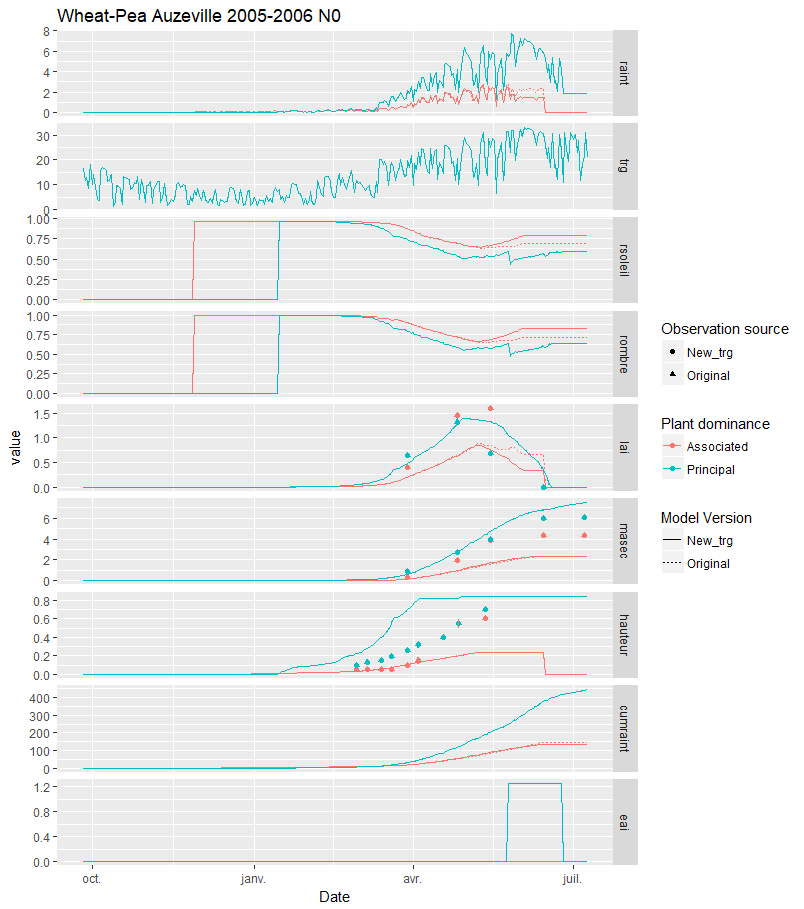
\includegraphics{img/trg-computation.png}

The comparison between both indicated that the dominated plant
intercepted more PAR with the original computation (\texttt{raint}), due
to its wrong light regime (\texttt{rsoleil} for both AS and AO). While
the dry mass and height of the dominated plant did not change, its lai
was previously higher on the end of the rotation, which increased the
\texttt{rsoleil} and \texttt{rombre} of the ground (shown as associated
ones). These simulations also showed that the wheat (dominant) eai was
highly overestimated, which will be fixed in the next simulations.

\chapter{Plant density and equivalent plant density}\label{plantdensity}

\section{Introduction}\label{introduction-1}

The plant density, which is related to the interrow distance, seems to
be an important formalism to describe the crop, and particularly for
mixed crops. Several computations are made to represent plant
competition in the STICS model, making the density effect a complex
process. Lets describe each step of the process to have a clearer
representation in mind.

\section{The density effect on LAI}\label{the-density-effect-on-lai}

In the model, the plant density is taken as a negative effect upon the
\texttt{LAI} growth as soon as a threshold of \texttt{LAI} is reached.
This threshold (\texttt{P\_laicomp}) represents the moment when the leaf
surface of a plant start becoming competitive for light against another
plant (from the same species or not). So whenever the \texttt{LAI} is
higher than \texttt{P\_laicomp}, the effect of the density
(\texttt{efdensite}) become closer to 0 (the effect is null when equal
to 1, and maximum at 0). This effect is computed as:
\(ef_{densite}=\min\left\{1.0\ ;\ e^{P_{adens}\cdot\frac{log(densiteequiv)}{P_{bdens}}}\right\}\)
or more simply:
\(ef_{densite}=\min\left\{1.0\ ;\ (\frac{densiteequiv}{P_{bdens}})^{P_{adens}}\right\}\)

\begin{quote}
Note: replace the equation in the model to simplify too ?
\end{quote}

Here is a plot representing the density effect along the equivalent
density:
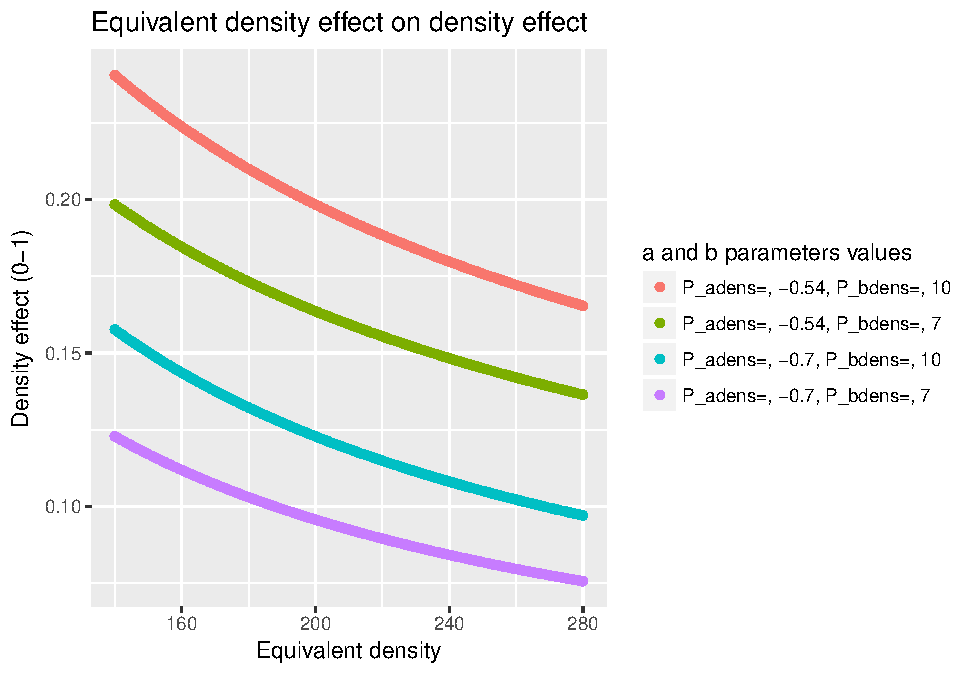
\includegraphics{Postdoc_steps_files/figure-latex/unnamed-chunk-12-1.pdf}

So the higher the density, the higher the negative effect on
\texttt{LAI}.

\section{The equivalent density}\label{the-equivalent-density}

In sole crops, the density effect is straightforward. However, under the
case of mixed crops, the density effect can be higher for the dominated
plant compared to its equivalent in sole crops. Indeed, a pea in sole
crop would have a given competition with other close plants, but a
different one when mixed with wheat, where the same density of wheat can
give higher competition effect for light because it is taller.

Then the density effect is computed as an equivalent density instead
(\texttt{densiteequiv}), that can differ from the sowing density for the
dominated crop to increase the negative effect of \texttt{efdensite}
compared to a sole crop.

The previous implementation in STICS was simple. The dominated plant had
a doubled equivalent density compared to its actual density. After some
discussion with the STICS intercrop team, Sebastian Munz modified the
STICS code to implement a new formalism to define the equivalent density
as a function of the height difference between the plants as follow:

\(density_{Equivalent} =\begin{cases}\Delta_{height} > hauteur_{threshold} & density_{p2} + \frac{density_{p1}}{P_{bdensp1}}\cdot P_{bdensp2} \\ \Delta_{height} < hauteur_{threshold} & density_{p2}+slope\cdot abs\left|\Delta_{height}\right| \end{cases}\)

with \(diffx= \frac{density_{p1}}{P_{bdensp1}}\cdot P_{bdensp2}\) and
\(slope= \frac{diffx}{hauteur_{threshold}}\)

Here is an exemple with a wheat-pea intercrop with a plant density of
140 for the wheat as the principal species and 30 for the pea as the
associated species:
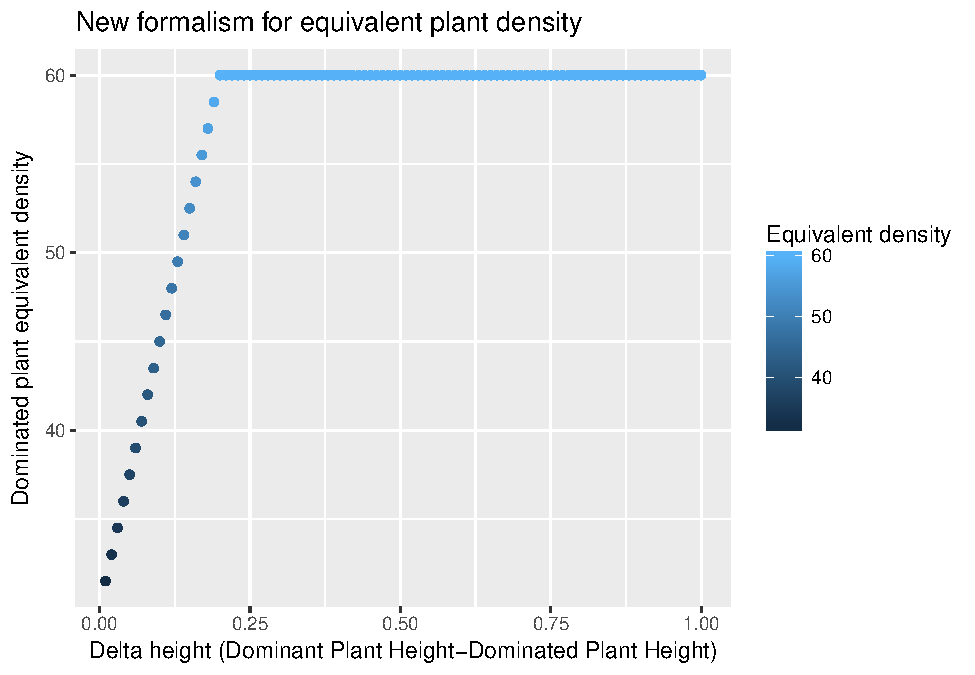
\includegraphics{Postdoc_steps_files/figure-latex/unnamed-chunk-14-1.pdf}

The new formalism has several implications in the model, notably that
the dominated plant is less impacted by the competition with the
dominant plant when both have approximately the same height.

A comparison of the two formalisms was made using the
\href{https://github.com/VEZY/sticRs}{sticRs} package, from which a
summary plot was extracted:
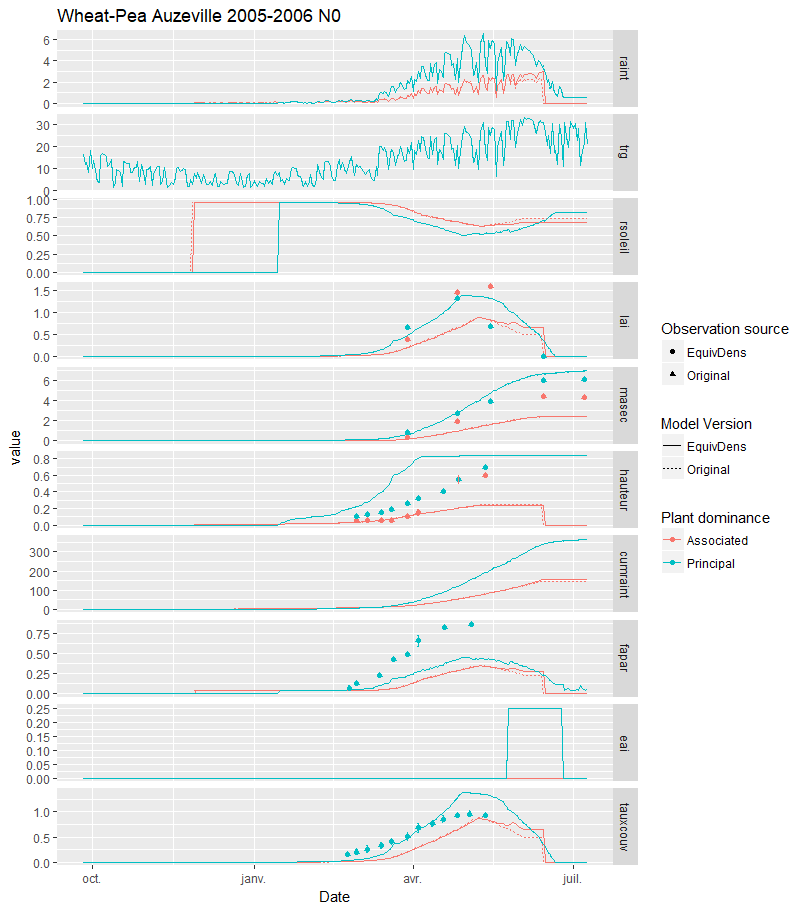
\includegraphics{img/Equ-dens-computation.png}

\chapter{Interrow spacing}\label{interrow-spacing}

\section{Introduction}\label{introduction-2}

The inter-row is the distance between two rows of the same plant
species. It is straightforward for monocrops, but a bit more informative
for intercrops. Indeed, the inter-row parameter can have unexpected
adverse effects for intercrops. Here is a simple design with a field
with two plant species sowed with the same inter-row:

\begin{figure}
\centering
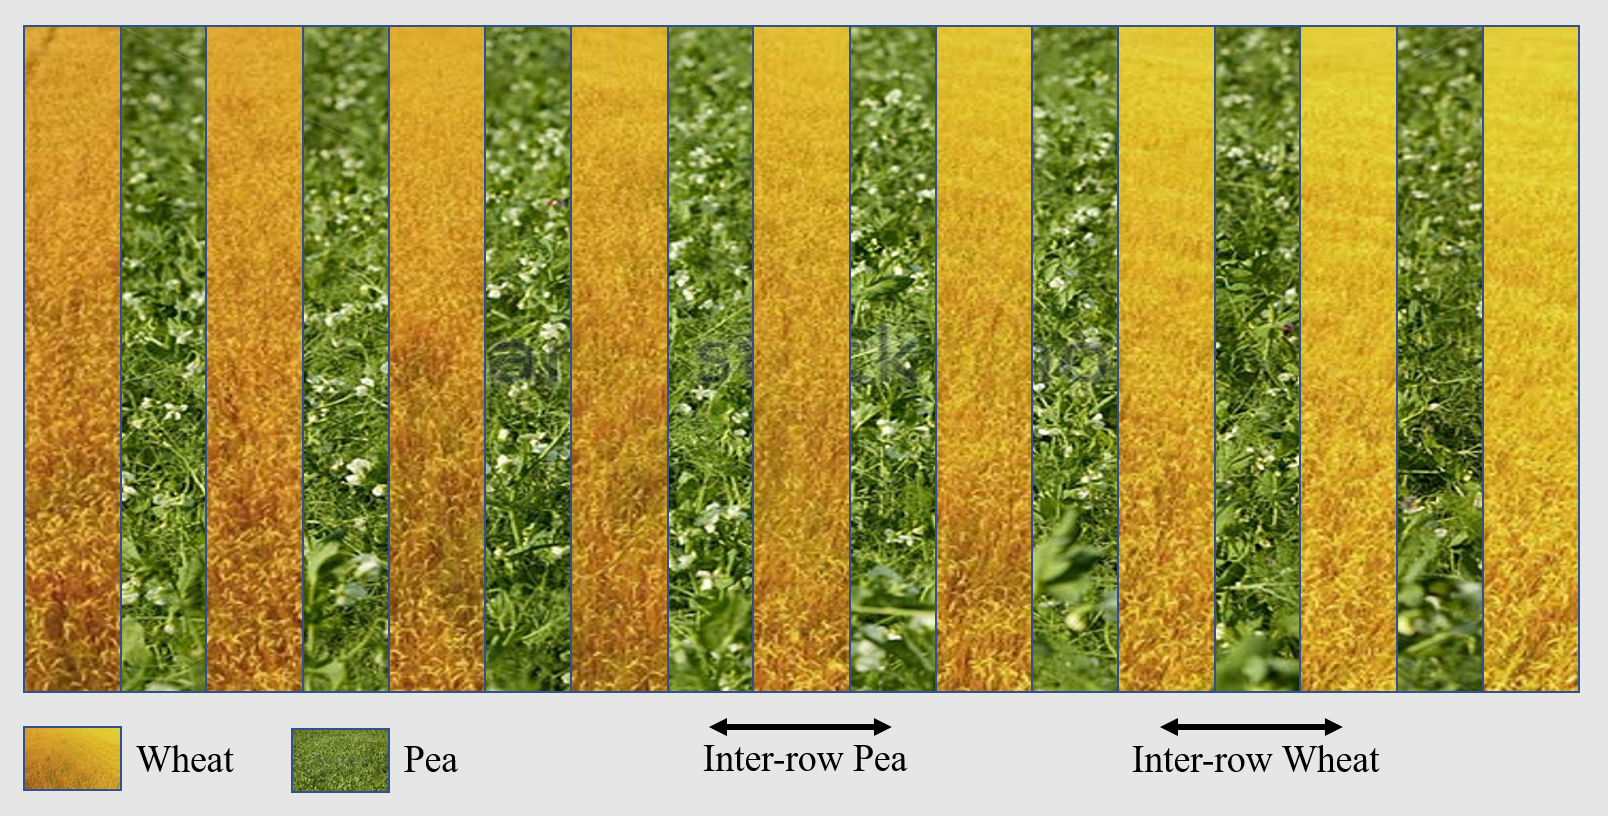
\includegraphics{img/Same-Interrow.png}
\caption{Pea-Wheat intercrop using the same inter-row spacing for the
two crops}
\end{figure}

So far, so good. Now what happens if we set a different inter-row
spacing for the two species ?

\section{Different inter-row spacing for mixed
crops}\label{different-inter-row-spacing-for-mixed-crops}

Note: look for \texttt{P\_interrang} in \texttt{rtrans} function (and
for \texttt{P\_orientrang} also) ; for \texttt{ir} in \texttt{rtrans}
function. Look also to the equivalent density in \texttt{croissance()}:

\bibliography{book.bib,packages.bib}


\end{document}
